%%%%%%%%%%%%%%%%%%%%%%%%%%%%%%%%%%%%%%%%%%%%%%%%%%%%%%%%%%%%%%%%%%%%
\begin{frame}[fragile]{A Short Course on C Language Programming}
\begin{itemize}
\item \href{mailto:Eidon@tutanota.com}{Eidon@tutanota.com}
\item Course slides at \url{https://github.com/Eidonko/ccourse}
\item Course software at 
\url{https://github.com/Eidonko}
\end{itemize}
\end{frame}

\begin{frame}[fragile]{Objectives}
Provide the audience with a set of
\begin{itemize}
\item ideas,
\item methods,
\item and know-how
resulting from several years of design and development
with the C language in an engineering environment.

\item Problem solving with C: syntactical analysis.
\end{itemize}

\end{frame}
\begin{frame}[fragile]{Purpose and structure}
\begin{itemize}
\item An introduction to C
\item The \texttt{FILE} methodology. Classes. Data hiding.
      Examples (class assoc, objalloc, vf\ldots)
\item Literate programming. The cweb tools
\item The GNU Autotools
\item Other classes for embedded systems (class tom, the ``art'' framework)
\item Linguistic support using C, Lex and YACC.
      Examples (the icgi interpreter, class FN, PvmLinda,
      the Ariel language...)
\item Exercise sessions, case studies, project works
\end{itemize}

%%The daily structure is on the net.
%%%%%%%%%%%%%%%%%%%%%%%%%%%%%%%%%%%%%%%%%%%%%%%%%%%%%%%%%%%%%%


%%%%%%%%%%%%%%%%%%%%%%%%%%%%%%%%%%%%%%%%%%%%%%%%%%%%%%%%%%%%%%
\end{frame}
\begin{frame}[fragile]{Advanced C Language for Engineering}

Exam: a project work (coding plus documentation) to be 
sent to me by the end of the year.

\vspace*{1cm}

%%%%%%%%%%%%%%%%%%%%%%%%%%%%%%%%%%%%%%%%%%%%%%%%%%%%%%%%%%%%%%

\end{frame}
\begin{frame}[fragile]{``The'' problem}
Teaching C to an audience with different backgrounds and
different expectations is very difficult.


\vspace{20pt}

Tuning the course is difficult.


\vspace{20pt}

Exercise sessions are particularly problematic.
\end{frame}

\begin{frame}[fragile]{Solutions}
Ideally, the course should be \emph{ad personam}.
Strong interaction with the teacher is
suggested. Just \href{mailto:Eidon@tutanota.be}{mail me} with your questions.


\vspace{20pt}

Practically speaking, exercises will be organized in 2 levels:
for those with no practical experience vs. for those with
practical experience.

\begin{itemize}
\item level A : for instance, learning how to log in a UNIX
	system, how to edit a C program, how to compile, and execute it
\item level B : designing ``improved'' versions, e.g., code optimisations;
writing test programs using the C classes at
\url{https://github.com/Eidonko}, and so forth.
\end{itemize}


\vspace{20pt}

For experienced people,
exercise sessions can be devoted to the design of the
solution of the project works.
\end{frame}

\begin{frame}[fragile]{Introduction to C: Structure}
\begin{itemize}
\item Introduction 
\item First examples
\item Fundamental data types, derived data types
\item Derived types: pointers and vectors
\item Functions
\item Structures and unions
\item Data hiding
\end{itemize}
%%}}}
\end{frame}

%%{{{  Introduction
%%%%%%%%%%%%%%%%%%%%%%%%%%%%%%%%%%%%%%%%%%%%%%%%%%%%%%%

\begin{frame}[fragile]{Introduction to C}
\begin{itemize}
\item C and UNIX : success stories.
\item C: developed by Ritchie to port UNIX from a PDP-7 to a PDP-11
\item System programming language
\item Most of the UNIX system is in C
\end{itemize}

%%%%%%%%%%%%%%%%%%%%%%%%%%%%%%%%%%%%%%%%%%%%%%%%%%%%%%%
\end{frame}
\begin{frame}[fragile]{Introduction to C}
\begin{itemize}
\item C is simple:
  \begin{itemize}
  \item A small number of simple and powerful instructions
  \item dealing with characters, numbers, addresses
  \item No language facilities for handling complex objects
        (strings, lists...)
  \item No language facilities for the I/O, for memory allocation...
  \end{itemize}
\item Those facilities are available as standard (or user-defined)
      libraries of functions
\end{itemize}
%%%%%%%%%%%%%%%%%%%%%%%%%%%%%%%%%%%%%%%%%%%%%%%%%%%%%%%
\end{frame}

\begin{frame}[fragile]{Introduction to C}
\begin{itemize}
\item C is small:
  \begin{itemize}
  \item Easy to describe, easy to learn
  \item The C compiler is considerably simple, compact-sized,
        and easy to write
\item The C data types and control structures often have
      a direct equivalent in the machine language of many
      computers. This happens because C was modelled after
      the machine language of the PDP 11. 
\item Hence, while in general the translation from a
      high level language instruction to machine language 
      is in general one-to-many, the translation from C
      to machine language is \textbf{one-to-few}.
\item A very simple run-time system: for instance (PDP-11)
         \index{PDP-11}:
   \begin{itemize}\item routines for 32-bit or 64-bit {\tt *} and {\tt /}.
      \item management of subroutine entry and exit.\end{itemize}
   \end{itemize}
\end{itemize}
\end{frame}
%%%%%%%%%%%%%%%%%%%%%%%%%%%%%%%%%%%%%%%%%%%%%%%%%%%%%%%

\begin{frame}[fragile]{Introduction to C}
C is portable\ldots

  \begin{itemize}
  \item but we need to follow some portability rules
  \item types have no well-defined size (e.g., in Python we have 
  	\texttt{numpy.int32}, in C we don't have an a-priori knowledge
	of the size of an \texttt{int})
  \item we can use symbolic constants for this
  \item large set of standard libraries for I/O, string manipulation,
  	memory allocation\ldots
  \end{itemize}

\end{frame}

%%%%%%%%%%%%%%%%%%%%%%%%%%%%%%%%%%%%%%%%%%%%%%%%%%%%%%%

\begin{frame}[fragile]{Introduction to C}
\parbox{1.0in}{BCPL\index{BCPL} \\ (typeless language\\by M. Richards)} $\Rightarrow$
\parbox{1.0in}{B Language\index{B Language} \\ (typeless lang.\\
 by K.  Thompson)} $\Rightarrow$
\parbox{1.0in}{C Language\\ (non-typeless,
 non-strongly-typed\index{Strongly-Typed Languages}
 language) by D. M.~Ritchie}

 \begin{description}
 \item[Typeless Language]: data are organized as multiple instances of the machine word.
 	Everything is allowed. Example: Assembly
 \item[Strongly-Typed\index{Strongly-Typed Languages} Language]: Nearly every
 	cast from type
 $A$ to type $B$ needs to be explicitly requested. Once a variable of a given type
 has been defined, also its
 {\em run-time checking\/} is defined in order to detect, e.g., overflow, underflow,
 subscript-out-of-range conditions, and so forth.
 ecc.  Examples: Pascal\index{Pascal}, Ada\index{Ada}.
 \end{description}


%%%%%%%%%%%%%%%%%%%%%%%%%%%%%%%%%%%%%%%%%%%%%%%%%%%%%%%
\end{frame}
\begin{frame}[fragile]{Introduction to C}
C is not a typeless language\index{Typeless Languages}: basic types are available
\begin{itemize}\item characters\item integers (in various sizes)
\item floating point numbers (in different sizes)
\item pointers\item facilities to build complex types from the basic types:
arrays\index{array}, records,
``unions\index{\tt union}'', functions.
\end{itemize}


\vspace{20pt}

C is not a strongly-typed\index{Strongly-Typed Languages} language:
it is {\em permissive\/}
about data casts. Its run-time executive does not cover
run-time checking.


%%%%%%%%%%%%%%%%%%%%%%%%%%%%%%%%%%%%%%%%%%%%%%%%%%%%%%%
\end{frame}
\begin{frame}[fragile]{Introduction to C}
C provides:
\begin{itemize}
\item the basic control-flow statements
    \begin{itemize} \item statement grouping
                    \item selective statements
                    \item iterative statements
    \end{itemize}
\item pointers\index{pointers} + {\em address arithmetic}
\end{itemize}

%%%%%%%%%%%%%%%%%%%%%%%%%%%%%%%%%%%%%%%%%%%%%%%%%%%%%%%
\end{frame}
\begin{frame}[fragile]{Introduction to C: Functions}
\begin{itemize}
\item Note:
     \begin{itemize}\item only call-by-value
                    \item recursion is allowed
                    \item single-level functions
                      that can be compiled separately.
                    \item variables
                      \begin{itemize} \item scope:
                                        ``blo\-ck-stru\-ctu\-red fashion''
			\item static vs. automatic
                      \end{itemize}
     \end{itemize}
\end{itemize}


%%%%%%%%%%%%%%%%%%%%%%%%%%%%%%%%%%%%%%%%%%%%%%%%%%%%%%%
\end{frame}
\begin{frame}[fragile]{Introduction to C}
\begin{verse}
 ``The only way to learn a new programming language is by writing
   programs in it; the first program to write is the same for all
   languages: print the words \texttt{"hello, world"}.'' [KR]

 ``What we have to learn to do we learn by doing.'' [Aristotle]
\end{verse}


\vspace{20pt}

\begin{verbatim}
           main()    /* prints "hello world." */
           {         /* and goes to the next line */
               printf("hello world.\n");
           }
\end{verbatim}

%%%%%%%%%%%%%%%%%%%%%%%%%%%%%%%%%%%%%%%%%%%%%%%%%%%%%%%
\end{frame}

\begin{frame}[fragile]{Introduction to C}
\begin{itemize}
\item Log into your Linux workstation\index{Linux}
\item type the {\tt "hello, world"} program
\item compile it
\item execute it
\end{itemize}



%%%%%%%%%%%%%%%%%%%%%%%%%%%%%%%%%%%%%%%%%%%%%%%%%%%%%%%
\end{frame}
\begin{frame}[fragile]{Introduction to C: a classic example}
\begin{verbatim}
/* The famous Fahrenheit to Celsius conversion :-) */
/* From the KC book! */
void main() {
    int inf, sup, step;
    float fahr, celsius;

    inf = 0;
    sup = 300;
    step = 20;

    fahr = inf;
    while  (fahr <= sup)  {
           celsius = (5.0/9.0) * (fahr-32.0);
           printf("%4.0f %6.1f\n", fahr, celsius);
           fahr = fahr + step;
    }
}
\end{verbatim}


%%%%%%%%%%%%%%%%%%%%%%%%%%%%%%%%%%%%%%%%%%%%%%%%%%%%%%%
\end{frame}
\begin{frame}[fragile]{Introduction to C}

Adapt the above code so to do the opposite
conversion.


\vspace{20pt}

Try to answer the following questions:
\begin{itemize}
\item why \verb"5.0/9.0" and not \verb"5/9"?
\item is \verb"5.0/9" equivalent to \verb"5.0/9.0"?
\item is the \verb".0" really necessary in \verb"fahr-32.0"?
\end{itemize}


%%%%%%%%%%%%%%%%%%%%%%%%%%%%%%%%%%%%%%%%%%%%%%%%%%%%%%%
\end{frame}
\begin{frame}[fragile]{Introduction to C: while loops}
\begin{verbatim}
while ( test ) action
\end{verbatim}


\vspace{20pt}

\verb"test" is executed. If output is non-zero (``true'') then
 \verb"action" is executed.

\vspace{20pt}


\verb"action" can also be a composite action
using curly brackets.


\vspace{20pt}

\begin{verbatim}
for (init; test; incr) action
\end{verbatim}

\noindent
is equivalent to
\begin{verbatim}
  init;
  while (test) { action; incr; }
\end{verbatim}


%%%%%%%%%%%%%%%%%%%%%%%%%%%%%%%%%%%%%%%%%%%%%%%%%%%%%%%
\end{frame}
\begin{frame}[fragile]{Introduction to C}

\verb"init", \verb"test", \verb"incr", and \verb"action" are all optional arguments: even
\begin{center}\tt for (;;) ;\end{center}
is allowed.

\vspace{20pt}

Note: \verb"test" is a {\em statement\/}!

\vspace{20pt}

Both {\tt while (a=3) ...} and {\tt while (a==3) ...} are valid!



%%%%%%%%%%%%%%%%%%%%%%%%%%%%%%%%%%%%%%%%%%%%%%%%%%%%%%%
\end{frame}
\begin{frame}[fragile]{Introduction to C}
Exercise: modify the previous example so to change the \verb"while" into \verb"for".

\vspace{20pt}

Exercise:  modify the previous example so to print the table in inverse order.


%%%%%%%%%%%%%%%%%%%%%%%%%%%%%%%%%%%%%%%%%%%%%%%%%%%%%%%
\end{frame}
\begin{frame}[fragile]{Introduction to C: conditional statements}
\begin{itemize}
\item statement ``if'':     \\
      if (condition) action${}_1$; else action${}_2$; \\
      (nesting and so forth.)
\item ``?:'' \\
      (condition)? action${}_1$ : action${}_2$;
\item ``switch'': \\
      switch(integer\_expr) \{  \\
      case value${}_1$: op${}_1$; break; \\
      case value${}_2$: op${}_2$; break; \\
      $\vdots$ \\
      case value${}_n$: op${}_n$; break; \\
      default: op${}_{n+1}$; \}
\end{itemize}


%%%%%%%%%%%%%%%%%%%%%%%%%%%%%%%%%%%%%%%%%%%%%%%%%%%%%%%
\end{frame}
\begin{frame}[fragile]{Introduction to C: loops and related statements}
\begin{itemize}
\item for
\item while
\item do while
\item break;
\item continue;
\item goto label
\end{itemize}


%%%%%%%%%%%%%%%%%%%%%%%%%%%%%%%%%%%%%%%%%%%%%%%%%%%%%%%
\end{frame}
\begin{frame}[fragile]{Introduction to C: defines and includes}
In C, it is possible to define symbolic constants via the \verb"#define"
pre-processor directive, and to specify that an external file should
be read in at compile time, via the \verb"#include"
pre-processor directive.


\vspace{20pt}

A few examples follow:

\begin{tabular}{||lll||} \hline\hline
\#define\index{\#DEFINE} & BEGIN & \{  \\
\#define & END   & \}  \\
\#define & IF    & if( \\
\#define & THEN  & ) \\
\#define & INT32 & long \\
\#define & INT32 & int \\
\#include & {\tt "file"} & \\
\#include & {\tt $<$file$>$} & \\ \hline\hline
\end{tabular}



%%%%%%%%%%%%%%%%%%%%%%%%%%%%%%%%%%%%%%%%%%%%%%%%%%%%%%%
\end{frame}
\begin{frame}[fragile]{Introduction to C: other pre-processor directives}
\begin{itemize}
\item macro substitution (e.g., {\tt \#define TRUE 1})
\item macro with parameters: \\
   \#define $MAX(a,b)\ \ ((A)>(B)$ ? $(A):(B))$ \\
   (Note: \#define sqr$(x)=$ $x*x$ is error-prone. Can you tell why?)
\item Conditional inclusion: ({\tt \#ifdef} and {\tt \#ifndef},
{\tt \#else} and {\tt \#endif}.)
\end{itemize}


%%%%%%%%%%%%%%%%%%%%%%%%%%%%%%%%%%%%%%%%%%%%%%%%%%%%%%%
\end{frame}
\begin{frame}[fragile]{Introduction to C: first functions for standard I/O}
\begin{itemize}
\item Defined in $<$stdio.h$>$
\item getchar (e.g. c=getchar()\index{I/O}), putchar (e.g. putchar(c)),
\EOF...
\end{itemize}


\vspace{20pt}

Example: copy of input to output --- version 1.


\vspace{20pt}

\begin{tt}
\begin{verbatim}
    #include <stdio.h>
    int main() { int c;
     c=getchar();
     while (c != EOF ) {
         putchar (c);
         c=getchar();
     }
    }
\end{verbatim}
\end{tt}



%%%%%%%%%%%%%%%%%%%%%%%%%%%%%%%%%%%%%%%%%%%%%%%%%%%%%%%
\end{frame}
\begin{frame}[fragile]{Introduction to C: first functions for standard I/O}
Example: copy of input to output --- version 2.


\vspace{20pt}

\begin{tt}
\begin{verbatim}
    #include <stdio.h>
    main() { int c;

    while ((c = getchar()) != EOF )
        putchar (c);
    }
\end{verbatim}
\end{tt}


\vspace{20pt}

Note: parentheses around \verb"c = getchar()" are necessary, because
of the larger priority of \verb"!=" with respect to \verb"=".



%%%%%%%%%%%%%%%%%%%%%%%%%%%%%%%%%%%%%%%%%%%%%%%%%%%%%%%
\end{frame}
\begin{frame}[fragile]{Introduction to C: first functions for standard I/O}
Exercise:
the just seen program can be easily adapted to work, e.g.,
as a ``word counter'' (reports the number of characters,
words, and lines in the input), or as a filter to remove blanks or
tabs, and so forth.


\vspace{20pt}

Input and output can be redirected with \verb"<" and \verb">".
Pipelines of programs can be built by chaining the programs with \verb"|".


%%%%%%%%%%%%%%%%%%%%%%%%%%%%%%%%%%%%%%%%%%%%%%%%%%%%%%%
\end{frame}
\begin{frame}[fragile]{Introduction to C: arrays}

To declare an array in C one has to use the following
syntax:

\vspace{20pt}

\begin{center}type name [dimension1][dimension2]..[dimension${}_n$] ;
\end{center} 


\vspace{20pt}

For instance, {\tt int vect[10];}


\vspace{20pt}

This is equivalent to e.g.
{\tt vect = numpy.array(10, dtype=numpy.int)}
in Python.


\vspace{20pt}


The index can be any integer expression.
  

\vspace{20pt}

There is no bound check like, e.g., in Ada.


%%%%%%%%%%%%%%%%%%%%%%%%%%%%%%%%%%%%%%%%%%%%%%%%%%%%%%%
\end{frame}
\begin{frame}[fragile]{Introduction to C: arrays}
Note: declaring an array means
\begin{enumerate}
\item declaring a \textbf{pointer}
\item and allocating memory for the pointed objects.
\end{enumerate}
The name of the array is indeed a pointer to the first element of the
array. In C lingo, this is written as
{\tt vect == \&vect[0]}. \label{arrayref}


\vspace{20pt}

Esercise: write a program, called report, that reports the occurrences of
each digit char in the input stream. Use an array of ten elements corresponding
to the ten decimal digits. Produce an histogram at end-of-input.

%%%%%%%%%%%%%%%%%%%%%%%%%%%%%%%%%%%%%%%%%%%%%%%%%%%%%%%
\end{frame}
\begin{frame}[fragile]{Introduction to C: arrays}
Exercise: use two programs, one that outputs the ten integer numbers
that count the occurrences of
each digit char in the input stream, the other one that creates a histogram
of its input values. Then use a pipeline to hook the two programs together.


\vspace{20pt}

\begin{center}
{\tt report2  |  histogram}
\end{center}



%%%%%%%%%%%%%%%%%%%%%%%%%%%%%%%%%%%%%%%%%%%%%%%%%%%%%%%
\end{frame}
\begin{frame}[fragile]{Introduction to C: functions}

Functions are named fragments of C code that can accept arguments and
return a value of some type.


\vspace{20pt}

Functions are, e.g., printf(), getchar()\index{I/O}, putchar(), main()\ldots\


\vspace{20pt}

No function hierarchy is allowed. The only ``special'' function is
main(). Functions can reside in a same source file or in more than one.



%%%%%%%%%%%%%%%%%%%%%%%%%%%%%%%%%%%%%%%%%%%%%%%%%%%%%%%
\end{frame}
\begin{frame}[fragile]{Introduction to C: functions}
Functions have the following structure: 


\vspace{20pt}

   {\tt [type]} {\em name\/} {\tt ( [ {\em args\/} ] ) }


   {\tt \{ [ {\em declarations\/} ] [ {\em instructions\/} ] \} }


\vspace{20pt}

\begin{tt}
\begin{verbatim}
  int main() {
      int i; int power (int, int);
      for (i=0; i<10; ++i)
          printf("%d %d\n", i, power(2,i));
  }
  int power (int x, int n) { int i, p;
    for (i = p = 1; i <= n; ++i)
       p=p*x;
    return (p);
  }
\end{verbatim}
\end{tt}
%%%%%%%%%%%%%%%%%%%%%%%%%%%%%%%%%%%%%%%%%%%%%%%%%%%%%%%
\end{frame}

\begin{frame}[fragile]{Introduction to C}

\texttt{return} closes the function and returns an output value
(default: integer) to the caller.


\vspace{20pt}

Arguments are passed \textbf{by value}: this means that
the arguments are copied in temporary variables.


\vspace{20pt}

The only way to let a function modify an argument is by passing
\emph{the address\/} of the object to be modified. 


\vspace{20pt}

Operator \verb"&" returns the address of a variable.


\vspace{20pt}

Note that, when you need to pass an array, passing its name is
indeed passing a pointer to the array.


%%%%%%%%%%%%%%%%%%%%%%%%%%%%%%%%%%%%%%%%%%%%%%%%%%%%%%%
\end{frame}
\begin{frame}[fragile]{Introduction to C: strings}
Strings are available in C as arrays of characters. Any sentence
enclosed between two \verb'"''s is an array of characters ending
with character \verb"'\0'" (NULL).


\vspace{20pt}

For instance, {\tt "hello"} $\Rightarrow$ 'h', 'e', 'l', 'l', 'o', 0


\vspace{20pt}

A very common mistake when learning C:

\begin{tt}
\begin{verbatim}
  char s1[10] = "Hello ";
  char s2[10] = "World";

  s1=s2;    /* ERROR */
\end{verbatim}
\end{tt}



%%%%%%%%%%%%%%%%%%%%%%%%%%%%%%%%%%%%%%%%%%%%%%%%%%%%%%%
\end{frame}
\begin{frame}[fragile]{Introduction to C}
As strings are arrays, we can easily pass a string to a function
by passing its name, which points to its characters:


\vspace{20pt}

\begin{verbatim}
  char a[] = "Pogo Possum";
  printf("Vote %s for president.\n", a);
  /* a = &a[0] */
\end{verbatim}


Variables defined within a function cannot be ``seen'' from other functions.

\vspace{20pt}


Two main classes of variables: {\tt automatic} vs. {\tt static}. Automatic variables
are allocated at function call and deallocated when the function stops.
They require initialisation. Static variables are allocated at compile time.
They are initialised to zero, and \emph{keep the value we left in them
when we get out of the functions where they are defined.}


%%%%%%%%%%%%%%%%%%%%%%%%%%%%%%%%%%%%%%%%%%%%%%%%%%%%%%%
\end{frame}
\begin{frame}[fragile]{Introduction to C}
\begin{itemize}
\item identifiers have the following structure:
      $<$alpha$>$ { $<$alphanum$>$ }*
\item six basic types: char, short, int, long, float, double.
\item qualifiers: unsigned, register
\item constants:
    \begin{itemize}
    \item scientific notation, e.g., {\tt 1.5e3} $\rightarrow$ double
    \item postfix notation, e.g., 145L $\rightarrow$ long
    \item prefix notation: '0x44' $\rightarrow$ unsigned int, hexadecimal, '044'
          $\rightarrow$ unsigned int, octal
    \item costant char. \verb"'c'" = character c  $\rightarrow$ char
\end{itemize}
\end{itemize}

%%%%%%%%%%%%%%%%%%%%%%%%%%%%%%%%%%%%%%%%%%%%%%%%%%%%%%%
\end{frame}
\begin{frame}[fragile]{Introduction to C}
    \begin{itemize}
    \item special constants, e.g., \verb"\n", \verb"\t", \verb"\0", \verb"\\", \verb'\"' and so forth  $\rightarrow$ char
    \item ``bit patterns'': \verb"\ddd", \verb"ddd" being an octal number.
    \item string constants, e.g., {\tt "string"} or {\tt ""}.
\end{itemize}


\vspace{20pt}

Exercise: write a function that counts the number of character
pointed by its string argument ({\tt strlen}).



%%%%%%%%%%%%%%%%%%%%%%%%%%%%%%%%%%%%%%%%%%%%%%%%%%%%%%%
\end{frame}
\begin{frame}[fragile]{Introduction to C: declarative instructions}
\begin{itemize}
\item Declarative instructions take the following form: \\
	\emph{typename list-of-variables;}
\item A declarative instruction can be followed
by an initialisation: \\
	int n=5; float g=5.4;
\item If the variable is an automatic one, then the initialisation is done
      \emph{each time the variable is allocated\/} (each time the function in which
      the variable resides is called).
\end{itemize}

%%%%%%%%%%%%%%%%%%%%%%%%%%%%%%%%%%%%%%%%%%%%%%%%%%%%%%%
\end{frame}
\begin{frame}[fragile]{Introduction to C: declarative instructions}
\begin{itemize}
\item Non-initialised automatic variables contain random value.
\item If the variable is a static one, then the initialisation is done
\emph{only once\/} (at compile time).
\item Static variables are always initialised. Default=0.
\item \emph{Global, static variables are only visible to the functions
      in the same source file}: this can be used for data hiding.
\end{itemize}



%%%%%%%%%%%%%%%%%%%%%%%%%%%%%%%%%%%%%%%%%%%%%%%%%%%%%%%
\end{frame}
\begin{frame}[fragile]{Introduction to C: operators}
\begin{itemize}
\item binary: +, -, $\ast$, /, \%
\item unary {\bf -}
\item precedences\index{precedenza}: +,- $<_{\rm prec}$ $\ast$,/,\% $<_{\rm prec}$ {\bf -}
\end{itemize}


\vspace{20pt}

\begin{itemize}
\item {\tt ||} \pre
\item \&\& \pre
\item == and !=, \pre
\item $>$ $>=$ $<$ $<=$
\end{itemize}


%%%%%%%%%%%%%%%%%%%%%%%%%%%%%%%%%%%%%%%%%%%%%%%%%%%%%%%
\end{frame}
\begin{frame}[fragile]{Introduction to C: operators}
Expressions such as:

\vspace{20pt}

\begin{center}
$i<lim$ \&\& (c=getchar()\index{I/O}) != '\\n' \&\& c != \EOF
\end{center}
do not require extra parentheses:
 =\pre !=, hence parentheses are required around
\verb"c=getchar()".


\vspace{20pt}

Logic clauses are evaluated left-to-right. Evaluation stops when the truth value
of a logic expression is ascertained.



%%%%%%%%%%%%%%%%%%%%%%%%%%%%%%%%%%%%%%%%%%%%%%%%%%%%%%%
\end{frame}
\begin{frame}[fragile]{Introduction to C: derived types}

The following operators define complex types derived from the
basic types of C:

\vspace{20pt}

\begin{description}
\item[\texttt{*}] operator pointer-to,
\item[\texttt{[]}] operator vector-of,
\item[\texttt{()}] operator pointer-to-function.
\end{description}

%%%%%%%%%%%%%%%%%%%%%%%%%%%%%%%%%%%%%%%%%%%%%%%%%%%%%%%
\end{frame}
\begin{frame}[fragile]{Introduction to C: derived types}
\begin{itemize}
\item \verb"char *p;" : \verb"p" is of type ``pointer-to-chars''
\item \verb"float v[10];" : \verb"v" is a vector, i.e., a pointer to the beginning of
  a memory area allocated by the system and consisting of 10 floats, i.e.,
  \verb"v[0]", \ldots, \verb"v[9]".
\item \verb"int getX();" : \verb"getX" is a pointer to a function returning an int.
\end{itemize}


%%%%%%%%%%%%%%%%%%%%%%%%%%%%%%%%%%%%%%%%%%%%%%%%%%%%%%%
\end{frame}
\begin{frame}[fragile]{Introduction to C: derived types}
Operator \verb"[]" has higher priority with respect to operator
\verb"*". This means that


\vspace{20pt}

\begin{center}
           \tt int *v[10]
\end{center}


\vspace{20pt}

\noindent means that \verb"v" is a vector of ten pointers-to-int.
Parentheses are necessary to change the meaning:


\vspace{20pt}

\begin{center}
           \tt int (*v)[10]
\end{center}

\noindent means that \verb"v" is a pointer to a vector of ten integers.


\vspace{20pt}

What's the difference in terms of sizes?


%%%%%%%%%%%%%%%%%%%%%%%%%%%%%%%%%%%%%%%%%%%%%%%%%%%%%%%
\end{frame}
\begin{frame}[fragile]{Introduction to C: derived types}
%%%%%%%%%%%%%%%%%%%%%%%%%%%%%%%%%%%%%%%%%%%%%%%%%%%%%%%
\begin{enumerate}
\item \verb"int *pi;" : pointer to integer;
\item \verb"char **argv;" : pointer to pointer-to-char;
\item \verb"float *(fvp)[5];" : pointer to vectors-of-5-floats
\item \verb"long (*fp)(int);" : pointer to function reading an int and returning a long.
\end{enumerate}

%%%%%%%%%%%%%%%%%%%%%%%%%%%%%%%%%%%%%%%%%%%%%%%%%%%%%%%
\end{frame}
\begin{frame}[fragile]{Introduction to C: derived types}
%%%%%%%%%%%%%%%%%%%%%%%%%%%%%%%%%%%%%%%%%%%%%%%%%%%%%%%
The address-of (\verb"&") operator returns the address of a variable.


\vspace{20pt}

\begin{verbatim}
char c; char *pc;   pc = &pc;
\end{verbatim}


\vspace{20pt}

Operator \verb"*", applied to a pointer, returns the pointed object.


\vspace{20pt}

\begin{verbatim}
char c1 = 'a';   char *p = &c1;
char c2 = *p2;   /* c2 == 'a' */
\end{verbatim}


\vspace{20pt}

\begin{verbatim}
void func(char *s) { printf("bye %s\n", s) }

main() { void (*pfunc)(char*) = func;
         *(pfunc)("hello");
     }
\end{verbatim}

%%%%%%%%%%%%%%%%%%%%%%%%%%%%%%%%%%%%%%%%%%%%%%%%%%%%%%%
\end{frame}
\begin{frame}[fragile]{Introduction to C: derived types}
%%%%%%%%%%%%%%%%%%%%%%%%%%%%%%%%%%%%%%%%%%%%%%%%%%%%%%%
Pointers solve the problem of the lack of ``call-by-reference''
in C functions. For instance, in order to realize a function that
swaps its argument, one may use the following strategy:


\vspace{20pt}

\begin{verbatim}
 int swap(int *a, int *b) { int t;
     t = *a,   *a = *b,    *b = t;
 }
\end{verbatim}


\vspace{20pt}

The caller then needs to specify the addresses of the operands (s)he wants to
swap, as in \verb"swap(&i, &j)".


%%%%%%%%%%%%%%%%%%%%%%%%%%%%%%%%%%%%%%%%%%%%%%%%%%%%%%%
\end{frame}
\begin{frame}[fragile]{Introduction to C: derived types}
%%%%%%%%%%%%%%%%%%%%%%%%%%%%%%%%%%%%%%%%%%%%%%%%%%%%%%%
Arrays and pointers are strictly related to each other:
In particular, if {\tt int a[10];}
then a $\equiv$ \&a[0], a+1 $\equiv$ \&a[1] and so forth.
In other words,
\begin{center}\tt *(a+i) $\equiv$ a[i] \end{center}


\vspace{20pt}

Any indexed array is equivalent to
a pointer plus some offset, and vice-versa.


\vspace{20pt}

Big difference: the array is a constant, i.e., it can never 
appear on the left hand side of the \verb"=" sign, as in
$$a=pa$$
or in
$$a++$$

%%%%%%%%%%%%%%%%%%%%%%%%%%%%%%%%%%%%%%%%%%%%%%%%%%%%%%%
\end{frame}
\begin{frame}[fragile]{Introduction to C: derived types}
%%%%%%%%%%%%%%%%%%%%%%%%%%%%%%%%%%%%%%%%%%%%%%%%%%%%%%%
When passing an array to a function
we are indeed passing the address of its first element; this
address is copied 
(call-by-value) in a temporary variable. This variable may be
a pointer.


\vspace{20pt}

Example:

\begin{verbatim}
   char s[7] = "hello!";  /* s is an array */
   int  i = strlen(s);

   int strlen (char *x) { /* x is a pointer */
      int n;
      for (n=0; *x; x++)  /* hence, can be modified */
         n++;
      return (n);
   }
\end{verbatim}



%%%%%%%%%%%%%%%%%%%%%%%%%%%%%%%%%%%%%%%%%%%%%%%%%%%%%%%
\end{frame}
\begin{frame}[fragile]{Introduction to C: address arithmetics}
%%%%%%%%%%%%%%%%%%%%%%%%%%%%%%%%%%%%%%%%%%%%%%%%%%%%%%%
If p is a pointer, p++ lets p point to the next item.
It is the language that takes care of moving p of the
right amount of memory.


\vspace{20pt}

For instance,
\begin{tabular}{lll}
\multicolumn{3}{c}{\Int$\equiv$ 2 byte} \\
int *p;      &   \&p = 1222    & \&(p++) = 1224 \\
\multicolumn{3}{c}{\Double$\equiv$ 8 byte} \\
double *p;   &   \&p = 5644    & \&(p++) = 5660 \\
\multicolumn{3}{c}{and so forth}
\end{tabular}


\vspace{20pt}

In other words:
if p is a pointer to an object of type t, then
p+n points n objects further and p-n points n objects before.
The actual size of the object doesn't matter.




\end{frame}
\begin{frame}[fragile]{Introduction to C: type casts}
Implicit type casts occur when, in expressions, operands belong to different types.  Conversions obey the following rules:

\vspace{20pt}

\begin{itemize}
\item \Char and \Short $\rightarrow$ \Int, \Float $\rightarrow$ \Double
\item if an operand is \Double{}, the other becomes \Double and the result is
\Double
\item otherwise, if an operand is \Long, the other becomes \Long and the result is a
\Long
\item  otherwise, if an operand is unsigned, the other one becomes unsigned
and the result is unsigned.
\item otherwise, operands and result are \Int.
\end{itemize}


%%%%%%%%%%%%%%%%%%%%%%%%%%%%%%%%%%%%%%%%%%%%%%%%%%%%%%%
\end{frame}
\begin{frame}[fragile]{Introduction to C: conversions}
Converting a string of digits into a number, and vice-versa,
requires specific support.
Functions are available for this, e.g., \verb"atoi()":


\vspace{20pt}

\begin{tt}
\begin{verbatim}
   int atoi(char s[]) { int i, n;
        n = 0;
        for (i=0; s[i]>='0' && s[i]<='9'; ++i)
            n=10*n + s[i] -'0';
        return (n);
   }
\end{verbatim}
\end{tt}


\vspace{20pt}

Note how expression  {\tt s[i] - '0'} converts numeric character
\verb"s[i]" into the digit it represents.


%%%%%%%%%%%%%%%%%%%%%%%%%%%%%%%%%%%%%%%%%%%%%%%%%%%%%%%
\end{frame}
\begin{frame}[fragile]{Introduction to C: conversions}
The following function can be used to convert an uppercase character
into its lowercase counterpart.


\vspace{20pt}

\begin{tt}
\begin{verbatim}
      lower(c)
      int c;
      {
        if (c >='A' && c <= 'Z')
           return (c + 'a' - 'A');
        else
           return (c);
      }
\end{verbatim}
\end{tt}


\vspace{20pt}

Note: this program only works for code tables in which \verb"'a'"
follows \verb"'A'". This is true with ASCII and false with other codes
(e.g., EBCDIC.)


%%%%%%%%%%%%%%%%%%%%%%%%%%%%%%%%%%%%%%%%%%%%%%%%%%%%%%%
\end{frame}
\begin{frame}[fragile]{Introduction to C: conversions}

Problem: the C language does not specify anything about the sign of a \Char.
Hence, when a \Char is converted to an \Int, the result may lead to 
a negative number.


\vspace{20pt}

A case of machine-dependance: for instance, on the PDP-11, a \Char{} is signed, hence
if a character has the MSB set to one it becomes a
negative integer when cast to \Int. On other platforms a \Char{}
is unsigned.


%%%%%%%%%%%%%%%%%%%%%%%%%%%%%%%%%%%%%%%%%%%%%%%%%%%%%%%
\end{frame}
\begin{frame}[fragile]{Introduction to C: conversions}
The most common problem related to this is due to the value of
the constant character \EOF, i.e., $-1$.
The following C code:


\vspace{20pt}

\begin{tt}
\begin{verbatim}
      char c;

      c=getchar();
      if (c == EOF) .....
\end{verbatim}
\end{tt}


\vspace{20pt}

is faulty when executed on platforms in which \Char is \UNS{}, because
by the conversion rules, $-1$ becomes 255 and the \verb"if" is never
true.


\vspace{20pt}

The problem is solved when we declare \verb"int c".


%%%%%%%%%%%%%%%%%%%%%%%%%%%%%%%%%%%%%%%%%%%%%%%%%%%%%%%
\end{frame}
\begin{frame}[fragile]{Introduction to C: conversions and types}

Sign of \EOF{} on some platforms:


\vspace{20pt}

\begin{tabular}{cccccc}
SUN3 & HP9K & AIX & T800 & MSDOS & VM\\
-1&-1&255&255&-1&255
\end{tabular}


\vspace{20pt}

\verb"sizeof"'s on those platforms:


\vspace{20pt}

\begin{tabular}{cccccccc}
 & SUN3 & HP9K & AIX & T800 & MSDOS & VM\\
short & 2&2&2&2&2&2\\
int & 4&4&4&4&2&2\\
long & 4&4&4&4&4&4\\
float & 4&4&4&4&4&4\\
double & 8&8&8&8&8&8
\end{tabular}

%%%%%%%%%%%%%%%%%%%%%%%%%%%%%%%%%%%%%%%%%%%%%%%%%%%%%%%
\end{frame}
\begin{frame}[fragile]{Introduction to C: conversions}

While in general, in C, zero means false and non-zero means true,
the truth value in expressions such as


\vspace{20pt}

\begin{tt}
\begin{verbatim}isdigit = c >= '0' && c <= '9';
\end{verbatim}
\end{tt}


\vspace{20pt}

is 1 for true and 0 for false.


%%%%%%%%%%%%%%%%%%%%%%%%%%%%%%%%%%%%%%%%%%%%%%%%%%%%%%%
\end{frame}
\begin{frame}[fragile]{Introduction to C: conversions}
\begin{center}Explicit cast\end{center}

The cast operator changes the type of an object.
For instance, the following expression:


\vspace{20pt}

\begin{verbatim}
           celsius = ( (double)5 /9) * (fahr-32.0);
\end{verbatim}


\vspace{20pt}

is equivalent to 


\vspace{20pt}

\begin{verbatim}
           celsius = (5.0/9.0) * (fahr-32.0);
\end{verbatim}


\vspace{20pt}

Casting is invoked by specifying a type between parentheses.



%%%%%%%%%%%%%%%%%%%%%%%%%%%%%%%%%%%%%%%%%%%%%%%%%%%%%%%
\end{frame}
\begin{frame}[fragile]{Introduction to C: increment/decrement operators}
\begin{center}
\parbox{3cm}{IN C: \\ int i = 0; \\ i++;} \hskip .3cm $\Rightarrow$
\hskip .3cm \parbox{5cm}{in Assembly:\\ DATA segment \\ i DB 0 \\ \vdots \\ INC i}
\end{center}


\vspace{20pt}

Operators such as \verb"++" or \verb"--" may have a direct
counterpart in the machine language. 



\vspace{20pt}

\begin{itemize}
\item Operator \verb"++"
increments the contents of a variable. $x=n++$ is \emph{not\/}
equivalent to $x=++n$.
\item Operator $--$ decrements the contents of a variable.
$x=n--$ is \emph{not\/} equivalent to $x=--n$.
\end{itemize}

%%%%%%%%%%%%%%%%%%%%%%%%%%%%%%%%%%%%%%%%%%%%%%%%%%%%%%%
\end{frame}
\begin{frame}[fragile]{Introduction to C: increment/decrement operators}
Esercise: function {\tt purge(char s[], int c)} removes all occurrences of \verb"c"
from \verb"s[]".


\vspace{20pt}

Esercise: functions  \verb"strcpy()" and \verb"strcat()".

%%%%%%%%%%%%%%%%%%%%%%%%%%%%%%%%%%%%%%%%%%%%%%%%%%%%%%%
\end{frame}
\begin{frame}[fragile]{Introduction to C: increment/decrement of pointers}
\begin{verbatim}
int strlen (char *p) { int i=0;
                       while (*p++) i++;
                       return i;
    }
\end{verbatim}


\vspace{20pt}

\verb"*p" returns the char pointed to by \verb"p".
\verb"*p++" does the same, but increments the pointer afterwards.


\vspace{20pt}

When does the while loop ends?

\end{frame}
\begin{frame}[fragile]{Introduction to C: increment/decrement of pointers}
This is an elternative way to write function \verb"strlen":
\begin{verbatim}
int strlen (char *p) { char *q = p;
                       while (*p++) ;
                       return q - p - 1;
    }
\end{verbatim}

%%%%%%%%%%%%%%%%%%%%%%%%%%%%%%%%%%%%%%%%%%%%%%%%%%%%%%%
\end{frame}
\begin{frame}[fragile]{Introduction to C: bitwise operators}
The following six operands can be applied to any integer expression:


\vspace{20pt}

\begin{description}
\item[\&] : bitwise AND
\item[{\tt |}] : bitwise OR
\item[\^{}] : bitwise exclusive OR
\item[$<<$] : left shift
\item[$>>$] : right shift
\item[\~{}] : unary complement.
\end{description}


%%%%%%%%%%%%%%%%%%%%%%%%%%%%%%%%%%%%%%%%%%%%%%%%%%%%%%%
\end{frame}
\begin{frame}[fragile]{Introduction to C: bitwise operators}
Bitwise AND can be used to set up ``masks'', e.g.,
\begin{center}\tt c = n \& 0177;
\end{center}
which zeroes all the bits from bit 8 onward. Bitwise OR
sets bits: 
{\tt x = x | MASK} sets to 1 the bits that are set in MASK.
$<<$ and $>>$ are respectively arithmetical shifts to the left and to the right
($\rightarrow$
multiplication resp. division by 2).


\vspace{20pt}

Operator \~{} turns each 1 into 0 and vice-versa; it is used in expressions
like, e.g.,
{\tt x \& \~ 077}, which zeroes the last bits of \verb"x".
Note that this is independent of the actual size of \verb"x", and
therefore it is ``more portable'' than, e.g.,
{\tt x \& 0177700}.



%%%%%%%%%%%%%%%%%%%%%%%%%%%%%%%%%%%%%%%%%%%%%%%%%%%%%%%
\end{frame}
\begin{frame}[fragile]{Introduction to C: bitwise operators}

\begin{tt}
\begin{verbatim}
    unsigned int
    MIDbit (unsigned int x,
            unsigned int start,
            unsigned int num)
    {
    return((x >> (start+1-num)) & ~(~0 << num));
    }
\end{verbatim}
\end{tt}


\vspace{10pt}

For instance,
MIDbit(x, 4, 3) returns the three bits at position 4, 3, and 2.
x $>>$ (p+1-n) shifts the bits of interest on the rightmost
position in the word.


\vspace{10pt}

{\tt \~{} 0} is 11...1; n shifts to left lead to
$11...1\underbrace{00..0}_{\rm n\ zeroes}$;


\vspace{10pt}

complementing this value
we get
$00...0\underbrace{11..1}_{\rm n\ ones}$.




%%%%%%%%%%%%%%%%%%%%%%%%%%%%%%%%%%%%%%%%%%%%%%%%%%%%%%%
\end{frame}
\begin{frame}[fragile]{Introduction to C: assignment operator}
In C lingo, the left part of an assignment is called an
lvalue, and the right part is called an rvalue:


\vspace{20pt}

\begin{center}
           lvalue = rvalue;
\end{center}


\vspace{20pt}

Expressions such as 

\begin{center}
           i = i + 2;
\end{center}


\vspace{20pt}

require two memory accesses to the same memory location,
which is referenced once in the lvalue and once in the rvalue.
In C, an equivalent expression is:


\vspace{20pt}

\begin{center}
            i += 2;
\end{center}


\vspace{20pt}

which does only one access.



\vspace{20pt}

(Of course, nothing prevents the compiler to catch an opportunity
for optimization here\ldots)


%%%%%%%%%%%%%%%%%%%%%%%%%%%%%%%%%%%%%%%%%%%%%%%%%%%%%%%
\end{frame}
\begin{frame}[fragile]{Introduction to C: assignment operator}

Binary operators


\vspace{20pt}

\begin{center}
$+$ $-$
$\ast$ / \% $<<$ $>>$ \& \^{} and {\tt |}
\end{center}


\vspace{20pt}

can use notation
$e_1$ op= $e_2$ instead of $e_1$ = $(e_1)$ op $(e_2)$.


\vspace{20pt}

Note that {\tt x *= y+1} is equivalent to {\tt x = x*(y+1)}.



\vspace{20pt}

An example follows:


\vspace{10pt}

\begin{tt}
\begin{verbatim}
    int bitcount(unsigned n) { int b;
       for (b=0; n != 0; n >>= 1)
           if (n & 01)
               b++;
       return (b);
    }
\end{verbatim}
\end{tt}

%%%%%%%%%%%%%%%%%%%%%%%%%%%%%%%%%%%%%%%%%%%%%%%%%%%%%%%
\end{frame}
\begin{frame}[fragile]{Introduction to C: assignment operator}

Let me consider the following two programs:


\vspace{20pt}

\begin{verbatim}
int main() { int n;           int main() { int n;
 n = 0;                        n = 0;
 n = n+2+n*n;                  n += 2+n*n;
}                             }
\end{verbatim}


\vspace{20pt}

When compiled with option \verb"-Qproduce .s" (on an old Sun3 workstation lol),
the output Assembly files differ in the following lines:

%%%%%%%%%%%%%%%%%%%%%%%%%%%%%%%%%%%%%%%%%%%%%%%%%%%%%%%
\end{frame}
\begin{frame}[fragile]{Introduction to C: assignment operator}
\begin{verbatim}
16,19c16,17
<       movl     a6@(-0x4),d1
<       addql    #0x2,d1
<       addl     d1,d0
<       movl     d0,a6@(-0x4)
---
>       addql    #0x2,d0
>       addl     d0,a6@(-0x4)
\end{verbatim}


\vspace{20pt}

(No differences with \verb"-O").

%%%%%%%%%%%%%%%%%%%%%%%%%%%%%%%%%%%%%%%%%%%%%%%%%%%%%%%
\end{frame}
\begin{frame}[fragile]{Introduction to C: assignment operator}

The assignment form {\bf op=}  is


\vspace{20pt}

\begin{itemize}
\item more efficient
\item more concise
\item closer to natural language: ``add 2 to i'' is much more
natural than ``take i, add 2 to it, and write the result back to i.''
\end{itemize}


\vspace{20pt}

Note that the assignment operator returns the rvalue.

%%%%%%%%%%%%%%%%%%%%%%%%%%%%%%%%%%%%%%%%%%%%%%%%%%%%%%%%%%%%%%
\end{frame}
\begin{frame}[fragile]{Pointers and arrays}
Function {\tt strcpy(char *a, char *b);}


\vspace{20pt}

Assumption: NULL-terminated strings. Note that NULL is (int)0,
i.e., ``false''


\vspace{20pt}

Function {\tt strcmp(char *s, char *t)}: returns a negative number if $s<t$,
0 if $s==t$, a positiven number if $s>t$.


\vspace{20pt}

\begin{tt}
\begin{verbatim}
  strcmp(char *s, char *t) {
     for ( ; *s == *t; s++, t++)
         if (*s == '\0') return (0);
     return (*s - *t);
  }
\end{verbatim}
\end{tt}

%%%%%%%%%%%%%%%%%%%%%%%%%%%%%%%%%%%%%%%%%%%%%%%%%%%%%%%%%%%%%%
\end{frame}
\begin{frame}[fragile]{Pointers and arrays}

Is this {\tt \#define} OK?
\begin{center}\tt
\#define STRCPY(a,b) while (*a++ = *b++) ;
\end{center}


%%%%%%%%%%%%%%%%%%%%%%%%%%%%%%%%%%%%%%%%%%%%%%%%%%%%%%%%%%%%%%
\end{frame}
\begin{frame}[fragile]{Pointers and arrays}
To declare multidimensional arrays one declares arrays of arrays.
For instance,


\vspace{20pt}

\begin{tt}
\begin{verbatim}
static int day_of_month[2][13] = {
 { 0, 31, 28, 31, 30, 31, 30, 31, 31, 30, 31, 30, 31},
 { 0, 31, 29, 31, 30, 31, 30, 31, 31, 30, 31, 30, 31} };
\end{verbatim}
\end{tt}


\vspace{20pt}

It is now possible to compute the day-of-year for a given
date, e.g., March 1st, 1991:
60${}^{\underline{\rm th}}$ day of year 1991.      \label{bisest}

%%%%%%%%%%%%%%%%%%%%%%%%%%%%%%%%%%%%%%%%%%%%%%%%%%%%%%%%%%%%%%
\end{frame}
\begin{frame}[fragile]{Pointers and arrays}
\begin{tt}
\begin{verbatim}
int day_of_year(int day, int month, int year)
{ int i, leap;

  leap = year%4 == 0 && year%100 != 0
          || year%400 == 0;
  for (i=1; i<month; i++)
      day += day_in_month[leap][i];
  return (day);
}
\end{verbatim}
\end{tt}


%%%%%%%%%%%%%%%%%%%%%%%%%%%%%%%%%%%%%%%%%%%%%%%%%%%%%%%%%%%%%%
\end{frame}
\begin{frame}[fragile]{Pointers and arrays}
\begin{itemize}
\item int v[i][j] \ \ vs. int v[i,j]
\item entries are stored ``by row'': the rightmost index is the
  one that varies the most when entries are referenced in the order
  they are stored.
\item initialisation: using curly brackets.
\item when passing a bidimensional array to a function,
      it is mandatory that the number of columns be specified.
For instance: \\
\verb"f(int day_in_month[2][13])", or \\
\verb"f(int day_in_month[][13])", or \\
\verb"f(int (*day_in_month)[13])", \\
i.e., pointer to array-of-13 integer entries.
\end{itemize}


%%%%%%%%%%%%%%%%%%%%%%%%%%%%%%%%%%%%%%%%%%%%%%%%%%%%%%%%%%%%%%
\end{frame}
\begin{frame}[fragile]{Pointers and arrays}
``Entries are stored by rows'' means that, e.g., 

\vspace{20pt}

\begin{center}
\tt int v[100][200];
\end{center}

\vspace{20pt}

is allocated the same way as a

\vspace{20pt}

\begin{center}
\tt int v[100 $\times$ 200];
\end{center}

\vspace{20pt}

i.e., as if it were a mono-dimensional array of 20000 int's.


%%%%%%%%%%%%%%%%%%%%%%%%%%%%%%%%%%%%%%%%%%%%%%%%%%%%%%%%%%%%%%
\end{frame}
\begin{frame}[fragile]{Pointers and arrays}

Fortran stores objects the opposite way with respect to C:

\begin{center}
for (i..) for (j..) a[i][j]
\end{center}

is equivalent to

\begin{center}
DO I.. DO J.. A(J,I)
\end{center}


\vspace{20pt}

Accessing element $(i,j)$ in a $n\times m$ matrix means accessing
element $k = i\times m + j$ in the associated mono-dimensional array.
The same applies for $N$-dimensional matrices, $N>2$.

%%%%%%%%%%%%%%%%%%%%%%%%%%%%%%%%%%%%%%%%%%%%%%%%%%%%%%%%%%%%%%
\end{frame}
\begin{frame}[fragile]{Pointers and arrays}
Note how, to compute value $k$ for an $N$ dimensional matrix
whose dimensions are $(d_1, d_2,\dots,d_N)$,
it is necessary to know the values $d_2, \ldots, d_N$:
\[k = f(d_2, \dots, d_N) \]


\vspace{20pt}

Note also that when we need to access sequencially all the elements
of a multidimensional matrix it is preferable to use a pointer
initialised to the first entry of the matrix.

%%%%%%%%%%%%%%%%%%%%%%%%%%%%%%%%%%%%%%%%%%%%%%%%%%%%%%%%%%%%%%
\end{frame}
\begin{frame}[fragile]{Pointers and arrays}
\begin{verbatim}
#define N 500
#define M 500
main() {
  int a[N][M];
  int i, j, c;
  int *pa = & (a[0][0]);
  int *pl = & (a[N-1][M-1]);

  while (pa < pl) {         for (i=0; i<N; i++)
     *pa = 0;                  for (j=0; j<M; j++) {
     c = *pa + 1;                a[i][j] = 0;
     *pa = c;                    c = a[i][j] +1;
     pa++;                       a[i][j] = c;
  }                            }
\end{verbatim}

%%%%%%%%%%%%%%%%%%%%%%%%%%%%%%%%%%%%%%%%%%%%%%%%%%%%%%%%%%%%%%
\end{frame}
\begin{frame}[fragile]{Pointers and arrays}

\begin{tabular}{lcc}
\textbf{HP9K} & 0.7--0.8 second & 1.2--1.3 seconds \\
\textbf{SUN3} & 1.1 seconds & 2.4 seconds
\end{tabular}


%%%%%%%%%%%%%%%%%%%%%%%%%%%%%%%%%%%%%%%%%%%%%%%%%%%%%%%%%%%%%%
\end{frame}
\begin{frame}[fragile]{Pointers and arrays}
Even when the access is not sequencial it is possible to
exploit specific access patterns (e.g., constant stride access).


\vspace{20pt}

An interesting alternative with respect to multidimensional
arrays is by using pointers.
For instance, the computational cost to access entry $(i,j)$ in
a $n\times m$ matrix is the one for computing multiplication
$(i*m)$ and addition $(\dots +j)$.


%%%%%%%%%%%%%%%%%%%%%%%%%%%%%%%%%%%%%%%%%%%%%%%%%%%%%%%%%%%%%%
\end{frame}
\begin{frame}[fragile]{Pointers and arrays}
If we change from


\vspace{20pt}

\begin{center}
\tt int a[100][100];
\end{center}

to

\begin{center}
\tt int** a;
\end{center}

\vspace{20pt}

and if we properly allocate the 100 pointers in the row and,
for each of them, the memory required for storing 100 int's,
then accessing entry $(i,j)$ means executing

\vspace{20pt}

\begin{center}
\tt *((*(a+i)+j))
\end{center}

\vspace{20pt}

that has a computational cost of only two additions.
Furthermore, no dimension information is required anymore
to access any element of the array.

%%%%%%%%%%%%%%%%%%%%%%%%%%%%%%%%%%%%%%%%%%%%%%%%%%%%%%%%%%%%%%
\end{frame}
\begin{frame}[fragile]{Array of pointers}
\begin{tt}
\begin{verbatim}
char *name_of_month (int n) {

 static char *names[] = {
     "illegal",
     "January",
     "February",
      .
      .
      .
     "December"
 };

 return ((n < 1 || n > 12)? names[0] : names[n] ;
}
\end{verbatim}
\end{tt}


%%%%%%%%%%%%%%%%%%%%%%%%%%%%%%%%%%%%%%%%%%%%%%%%%%%%%%%%%%%%%%
\end{frame}
\begin{frame}[fragile]{Pointers and arrays}
Argc and argv: a mechanism that allows a program
to inspect the strings on the command line.


\vspace{20pt}

For instance, command {\tt echo}:


\vspace{20pt}

\begin{tt}
\begin{verbatim}
   main(int argc, char *argv[]) {
    while (--argc > 0)
      printf("%s%c", *++argv, (argc>1)?' ':'\n' );
   }
\end{verbatim}
\end{tt}


\vspace{20pt}

Exercise: {\tt compute 2 3 4 + *} (in inverse Polish notation).

\vspace{20pt}


Exercise: write a function that associates user functions to
the command options.

%%%%%%%%%%%%%%%%%%%%%%%%%%%%%%%%%%%%%%%%%%%%%%%%%%%%%%%%%%%%%%
\end{frame}
\begin{frame}[fragile]{Pointers and arrays}

Exercise: write a function that sorts the entries of
an array of integers. Modify the function so that
it requires a pointer-to-function,
int (*confr)(int,int), to realize sortings in increasing vs.
decreasing order. 


\vspace{20pt}

Exercise: ``opaque'' function, working with pointers to object of
unknown size.


\vspace{20pt}

Exercise (array of functions): design a scanner of
a simple grammar. Tokens must correspond to the entries
in an array of functions.


%%%%%%%%%%%%%%%%%%%%%%%%%%%%%%%%%%%%%%%%%%%%%%%%%%%%%%%%%%%%%%
\end{frame}
\begin{frame}[fragile]{Structures}
Keyword {\tt struct} defines a ``record.''
An example follows:

\vspace{20pt}


\begin{tt}
\begin{verbatim}
        struct cd {
            char author[30];
            int year;
            char producer[20];
        };
\end{verbatim}
\end{tt}


\vspace{20pt}

This is a declaration of a \emph{type}: no element
of this type has been defined so far. No memory
has been allocated. It is now possible to declare
objects of type {\tt struct cd} :
\begin{center}\tt struct cd x, y, z;\end{center}


%%%%%%%%%%%%%%%%%%%%%%%%%%%%%%%%%%%%%%%%%%%%%%%%%%%%%%%%%%%%%%
\end{frame}
\begin{frame}[fragile]{Structures}
The members of a 
{\tt struct} can be accessed via operator
{\tt .}. For instance, in function on page~\ref{bisest}:


\vspace{20pt}

\begin{tt}
\begin{verbatim}
   struct cd d;

   leap = d.year%4 == 0 &&
               d.year%100 != 0 ||
               d.year%400 == 0;
\end{verbatim}
\end{tt}


\vspace{20pt}

Nesting of structures is allowed:
{\tt struct a \{ struct disco c; \} d;}


\vspace{20pt}

Access: {\tt d.c.year}.


\vspace{20pt}

Typedefs.

%%%%%%%%%%%%%%%%%%%%%%%%%%%%%%%%%%%%%%%%%%%%%%%%%%%%%%%%%%%%%%
\end{frame}
\begin{frame}[fragile]{Structures}
A pointer to a structure can be declared, e.g., as follows:
{\tt struct disco *a;}

Access:
{\tt (*a).year};

\begin{center}\tt
(*a).year $\equiv$ a-$>$year
\end{center}


%%%%%%%%%%%%%%%%%%%%%%%%%%%%%%%%%%%%%%%%%%%%%%%%%%%%%%%%%%%%%%
\end{frame}
\begin{frame}[fragile]{Structures}

Arrays of structures:
\begin{tt}
\begin{verbatim}
  struct key {
     char *keyword;
     int  keycount;
  } keytab[100];
\end{verbatim}
\end{tt}


%%%%%%%%%%%%%%%%%%%%%%%%%%%%%%%%%%%%%%%%%%%%%%%%%%%%%%%%%%%%%%
\end{frame}
\begin{frame}[fragile]{Structures}
Initialisation:


\vspace{20pt}

\begin{tt}
\begin{verbatim}
  struct key Keywords[] = {
         "break", 0,
         "case", 0,
         "char", 0,
         .
         .
         "while", 0
  };
\end{verbatim}
\end{tt}


%%%%%%%%%%%%%%%%%%%%%%%%%%%%%%%%%%%%%%%%%%%%%%%%%%%%%%%%%%%%%%
\end{frame}
\begin{frame}[fragile]{Structures}
Write a program that writes a static arrays of structs to be used
as look-up table for another program.


\vspace{20pt}

Structures can reference themselves:


\vspace{10pt}

\begin{tt}
\begin{verbatim}
    struct tnode {
      char *word; int count;
      struct tnode *left;
      struct tnode *right;
    };
\end{verbatim}
\end{tt}


\vspace{10pt}

or

\vspace{10pt}

\begin{tt}
\begin{verbatim}
    struct nlist {
      char *name; char *def;
      struct nlist *next;
    };
\end{verbatim}
\end{tt}

%%%%%%%%%%%%%%%%%%%%%%%%%%%%%%%%%%%%%%%%%%%%%%%%%%%%%%%%%%%%%%
\end{frame}
\begin{frame}[fragile]{Structures: bitfields}
Flag registers:


\vspace{20pt}

\begin{tt}
\begin{verbatim}
  #define KEYWORD  01
  #define EXTERN   02
  #define STATIC   04
  #define AUTOMT  010
   .
   .
  flags |= EXTERN | STATIC;
   .
  if ( flags & (EXTERN | STATIC) ) ...
\end{verbatim}
\end{tt}


\vspace{20pt}

It is possible to store in a same variable, {\tt flags}, a series
of conditions that can be ``turned on'' through a bitwise OR
{\tt |} and can be tested via the bitwise
AND {\tt \&}. Clearly the definitions must be powers of 2.
Octal implies {\tt unsigned}.



%%%%%%%%%%%%%%%%%%%%%%%%%%%%%%%%%%%%%%%%%%%%%%%%%%%%%%%%%%%%%%
\end{frame}
\begin{frame}[fragile]{Structures: bitfields}
Structures can be used to specify flag registers via so-called
``bitfields'':


\vspace{20pt}

\begin{tt}
\begin{verbatim}
  struct {
    unsigned is_keyword : 1;
    unsigned is_extern  : 1;
    unsigned is_static  : 1;
    unsigned is_regist  : 1;
  } flags;
\end{verbatim}
\end{tt}


\vspace{20pt}

Accessing a field: standard way ({\tt .} operator). For instance:
{\tt flags.is\_extern}.

%%%%%%%%%%%%%%%%%%%%%%%%%%%%%%%%%%%%%%%%%%%%%%%%%%%%%%%%%%%%%%
\end{frame}
\begin{frame}[fragile]{Structures: bitfields}
Bitfields can be used as lvalues and rvalues as any other
integer variable. This means that bitwise OR's and AND's
are not necessary:


\vspace{20pt}

\begin{center}\tt flags.is\_extern = 0\end{center}
\begin{center}\tt if (flags.is\_extern == 0) ...\end{center}


%%%%%%%%%%%%%%%%%%%%%%%%%%%%%%%%%%%%%%%%%%%%%%%%%%%%%%%%%%%%%%
\end{frame}
\begin{frame}[fragile]{Structures: bitfields}
\begin{itemize}
\item Bitfields can only be {\tt unsigned} or
{\tt int}
\item {\em Asking the address of a bitfield is illegal}
\item Bitfields can also be ``unnamed,'' e.g., for padding
\item The standard doesn't specify if MSB-first or LSB-first is used.
\end{itemize}


%%%%%%%%%%%%%%%%%%%%%%%%%%%%%%%%%%%%%%%%%%%%%%%%%%%%%%%%%%%%%%
\end{frame}
\begin{frame}[fragile]{Unions}
An {\tt union} is a variable having many identifiers associated to it.
These identifiers may be of different type and hence
different \verb"sizeof"'s. Each identifier refer
to the same amount of memory, i.e., as many bytes as the
``largest'' type requires.
For instance:


\vspace{20pt}

\begin{tt}
\begin{verbatim}
   union point_x {
     char   *pc;
     float  *pf;
     double *pd;
     long    regarded_as_an_int;
   } object;
\end{verbatim}
\end{tt}


%%%%%%%%%%%%%%%%%%%%%%%%%%%%%%%%%%%%%%%%%%%%%%%%%%%%%%%%%%%%%%
\end{frame}
\begin{frame}[fragile]{Unions}
Variable {\em object\/} has many ``aliases'': it can be regarded as
a pointer-to-char, if referred to as {\tt object.pc}, or as
pointer-to-double ({\tt object.pd}), or as a long
({\tt object.regarded\_as\_an\_int}). The amount of memory is always the
same, the one that is enough in order to store the ``largest'' among
a (char*), a (float*), a (double*), or a (long).


%%%%%%%%%%%%%%%%%%%%%%%%%%%%%%%%%%%%%%%%%%%%%%%%%%%%%%%%%%%%%%
\end{frame}
\begin{frame}[fragile]{Unions}
Typical use of unions:


\vspace{20pt}

\begin{tt}
\begin{verbatim}
  struct {
     int its_type;
     union {
         int    ival;
         float  fval;
         char  *pval;
     } uval;
  } symbol_table[500];
\end{verbatim}
\end{tt}


\vspace{20pt}

If we store in
{\tt symbol\_table[$i$].its\_type} a code that represents the {\em type\/} of object
$i$, then we can set up, e.g., arrays of objects of different types,
or linked lists of different objects, and so forth.


%%%%%%%%%%%%%%%%%%%%%%%%%%%%%%%%%%%%%%%%%%%%%%%%%%%%%%%%%%%%%%
\end{frame}
\begin{frame}[fragile]{Unions}
A {\tt switch} on {\tt its\_type} is the typical way to execute
diverse actions depending on the nature of the current object,
as it's done in the following excerpt:


\vspace{20pt}

\begin{tt}
\begin{verbatim}
  for (i=0;i<500;++i)
    switch(symbol_table[i].its_type) {
      case 'i': printf("%d",
                symbol_table[i].uval.ival);
                break;
        .
        .
    }
\end{verbatim}
\end{tt}


%%%%%%%%%%%%%%%%%%%%%%%%%%%%%%%%%%%%%%%%%%%%%%%%%%%%%%%%%%%%%%
\end{frame}
\begin{frame}[fragile]{Typedef}
The typedef statement can be used to define new types
without having to use cumbersome and long definitions. For
instance,


\vspace{20pt}

\begin{center}\tt typedef int LENGTH;\end{center}
defines a type alias for {\tt int} called {\tt LENGTH}.
Another simple example:


\vspace{20pt}

\begin{center}\tt typedef char *STRING;\end{center}


\vspace{20pt}

After this typedef the programmer can choose freely to
define a pointer-to-char either via
{\tt char *} or with {\tt STRING}.


%%%%%%%%%%%%%%%%%%%%%%%%%%%%%%%%%%%%%%%%%%%%%%%%%%%%%%%%%%%%%%
\end{frame}
\begin{frame}[fragile]{Typedef}
Typedef's are useful when types get complex and their
definitions longer. For instance,
type ``pointer-to-function returning an {\tt int}'' can be
aliased as follows:
\begin{center}\tt typedef int (*PFI)();\end{center}


\vspace{20pt}

Then, for instance, {\tt PFI strcmp, swap;} is equivalent to
\begin{center}\tt int (*strcmp)(), (*swap)();\end{center}



%%%%%%%%%%%%%%%%%%%%%%%%%%%%%%%%%%%%%%%%%%%%%%%%%%%%%%%%%%%%%%
\end{frame}
\begin{frame}[fragile]{Typedef}
There are two valid reasons for encouraging the use of
{\tt typedef}:
\begin{itemize}
\item parametrizing a program with its types may turn into semplifying
the solution of portability problems:
for instance,
\begin{center}\tt typedef short integer;\end{center}
Moving the code to a machine where the role of short is played by int
we only need to change one line of code:
\begin{center}\tt typedef int integer;\end{center}\index{tipi a grandezza definita}
\item enhancing a program's readability: a type called {\tt LENGTH} brings
with its name also a hint at its usage and meaning within the program.
\end{itemize}


%%%%%%%%%%%%%%%%%%%%%%%%%%%%%%%%%%%%%%%%%%%%%%%%%%%%%%%%%%%%%%
\end{frame}
\begin{frame}[fragile]{Input and output}
In C many functions are defined in the so-called ``standard library'',
\verb"libc.a". A set of headers refer to the functions
and definitions in the standard library. The header file
\verb"stdio.h" contains the basic functions and definitions for I/O:
\begin{center}\tt \#include $<$stdio.h$>$\end{center}


%%%%%%%%%%%%%%%%%%%%%%%%%%%%%%%%%%%%%%%%%%%%%%%%%%%%%%%%%%%%%%
\end{frame}
\begin{frame}[fragile]{Input and output}
C and UNIX define three standard I/O streams:
\begin{itemize}
\item {\tt stdin}, i.e., the standard input stream,
normally given by the characters typed at the keyboard.
As in DOS, the redirection character $<$ allows to
specify an alternative standard input stream as follows:
\begin{center}\tt prog $<$ inputfile\end{center}
\item {\tt stdout}, the standard output stream, normally given by the characters
typed onto our display.
Character $>$ redirects stdout on an other file, as in
{\tt prog $>$ outputfile}.
\item {\tt stderr}, the standard error stream, is again by default
our display. Is the stream where the programmer does (should) send
the error messages. Can be redirected via  $2>$, e.g.,
{\tt prog 2$>$ /dev/null}.
\end{itemize}


%%%%%%%%%%%%%%%%%%%%%%%%%%%%%%%%%%%%%%%%%%%%%%%%%%%%%%%%%%%%%%
\end{frame}
\begin{frame}[fragile]{Input and output}
Besides the stream redirection facilities, UNIX provides
the concept of  {\em pipe\/}: if we type
\begin{center}\tt prog${}_1$ | prog${}_2$\end{center}
the {\tt stdout} of prog${}_1$ becomes the {\tt stdin} of prog${}_2$.


%%%%%%%%%%%%%%%%%%%%%%%%%%%%%%%%%%%%%%%%%%%%%%%%%%%%%%%%%%%%%%
\end{frame}
\begin{frame}[fragile]{Input and output}
Pipes are also available as C functions:
for instance, 
\begin{center}\tt FILE *popen(const char *command, const char *type);\\
int pclose (FILE *stream);
\end{center}
the popen() function creates a pipe between the calling program
and  the  command  to  be  executed.
\verb"command"
consists  of  a  shell  command  line.  \verb"type" is an I/O mode,
either r for reading or w for writing.  The  value  returned
is  a stream pointer such that one can write to the standard
input of the command, if the I/O mode is w,  by  writing  to
the  file  stream; and one can read from the
standard output of the command, if the I/O  mode  is  r,  by
reading  from  the  file  stream.


%%%%%%%%%%%%%%%%%%%%%%%%%%%%%%%%%%%%%%%%%%%%%%%%%%%%%%%%%%%%%%
\end{frame}
\begin{frame}[fragile]{Input and output}
\begin{center}
FILE *f = popen("date", "r");\\
FILE *g=popen("/bin/sort", "w");
\end{center}

\vspace{20pt}

with the first one we can, e.g., read the output of command \verb"date".
The second one connects to service \verb"/bin/sort" so to
ask the service of an external command.



%%%%%%%%%%%%%%%%%%%%%%%%%%%%%%%%%%%%%%%%%%%%%%%%%%%%%%%%%%%%%%
\end{frame}
\begin{frame}[fragile]{Input and output}
\begin{center}\tt printf() \end{center}

printf() converts, formats and prints its arguments (except the
first one, a format string).
The format string consists of two classes of objects:
characters, that are simply copied onto stdout, and
conversion strings, each of which controls the conversion and
the printing of a further argument to printf().


\vspace{20pt}

Conversion strings start with
character {\tt \%} and end with a 
{\em conversion character\/}. Between {\tt \%} and the conversion character
there can be:

%%%%%%%%%%%%%%%%%%%%%%%%%%%%%%%%%%%%%%%%%%%%%%%%%%%%%%%%%%%%%%
\end{frame}
\begin{frame}[fragile]{Input and output}
\begin{itemize}
\item a hyphen, which implies left adjustment of the argument
convertito
\item a number specifying the minimum size of the output
\item a ``dot'' character, separating the previous numerical field from\ldots
\item a number that specifies either the maximum number of
characters that we can print from a string, or the number of decimal digits
in a float or double.
\item an {\tt l} that means long integer.
\end{itemize}


%%%%%%%%%%%%%%%%%%%%%%%%%%%%%%%%%%%%%%%%%%%%%%%%%%%%%%%%%%%%%%
\end{frame}
\begin{frame}[fragile]{Input and output}
Conversion characters:
\begin{description}
\item[d] decimal
\item[o] unsigned octal
\item[x] unsigned hexadecimal
\item[u] unsigned decimal
\item[c] character
\end{description}
%%%%%%%%%%%%%%%%%%%%%%%%%%%%%%%%%%%%%%%%%%%%%%%%%%%%%%%%%%%%%%

\end{frame}
\begin{frame}[fragile]{Input and output}
Conversion characters:
\begin{description}
\item[s] string
\item[e] float or double printed in ``scientific'' notation
\item[f] ditto, decimal notation
\item[g] as {\bf f}.
\end{description}


\vspace{20pt}

(several other conversion characters exist.)

%%%%%%%%%%%%%%%%%%%%%%%%%%%%%%%%%%%%%%%%%%%%%%%%%%%%%%%%%%%%%%
\end{frame}
\begin{frame}[fragile]{Input and output}
\begin{center}\tt scanf(formato, args...)\end{center}
scanf() is the dual function of printf(): it reads characters from stdin
and interprets and converts them according to what specified in
its first argument, writing results into the following
arguments.
{\em These arguments must be (valid) pointers!}


\vspace{20pt}

\begin{tt}
\begin{verbatim}
 int i;   float f;   char name[50];

 scanf("%d  %f  %s", &i, &x, name);
\end{verbatim}
\end{tt}


\vspace{20pt}

Given input: {\tt 25  54.32E-1 Thompson} {\em $<$return$>$\/}
the program associates 25 to {\tt i}, 5.432 to {\tt f} 5.432
and string {\tt "Thompson"} to {\tt name}.
%%}}}






%%{{{  The FILE Methodology
%%%%%%%%%%%%%%%%%%%%%%%%%%%%%%%%%%%%%%%
\end{frame}
\begin{frame}[fragile]{The FILE Methodology}
General idea:
\begin{itemize}
\item The user declares a pointer to an abstract entity called FILE:
\begin{center}
	FILE *f;
\end{center}
\item FILE can be seen as a \emph{service}: the user must
open a connection, send requests, receive replies, and close the
connection in order to interact with that service.
\item The user does not see the shape of the FILE struct; (s)he only
sees its interface.
\end{itemize}

%%%%%%%%%%%%%%%%%%%%%%%%%%%%%%%%%%%%%%%%%%%%%%%%%%%%%%%
\end{frame}
\begin{frame}[fragile]{The FILE Methodology}
\begin{itemize}
\item The user connects to the service via function fopen:
\begin{center}
	FILE *f; f = fopen("myfile", "r+");
\end{center}
\item Then the user sends requests to the service and gets replies
from it:
\begin{center}
	n = fread(myptr, sizemyobj, num\_elems, f);
	if (n == num\_elems) ...
\end{center}
\item Finally, the user disconnects:
\begin{center}
	fclose(f);
\end{center}
\end{itemize}

%%%%%%%%%%%%%%%%%%%%%%%%%%%%%%%%%%%%%%%%%%%%%%%%%%%%%%%
\end{frame}
\begin{frame}[fragile]{How to create a new FILE-like class}
Example: class ASSOC
\begin{itemize}
\item Associative arrays: a mechanism with which one creates
an \emph{association\/} between two entities.
\item A special class is the standard array, which sets up an
association between integers and C objects:
\begin{itemize}
\item double d[5];
\end{itemize}
\item $0\Rightarrow\mbox{*d}, \dots, i\Rightarrow\mbox{*(d+i)}, \dots$
\end{itemize}

%%%%%%%%%%%%%%%%%%%%%%%%%%%%%%%%%%%%%%%%%%%%%%%%%%%%%%%
\end{frame}
\begin{frame}[fragile]{How to create a new FILE-like class}
\begin{itemize}
\item Associative arrays create associations between any two
objects.
\item ASSOC creates association between any two \emph{pointers}.
\item ``url0'' $\Rightarrow$ ``https://github.com/Eidonko'':
(char*) $\Rightarrow$ (char*)
\item ``cos''  $\Rightarrow$ cos():
(char*) $\Rightarrow$ (double(*)())
\item ``myfile'' $\Rightarrow$ f:
(char*) $\Rightarrow$ (FILE*)
\end{itemize}

%%%%%%%%%%%%%%%%%%%%%%%%%%%%%%%%%%%%%%%%%%%%%%%%%%%%%%%
\end{frame}
\begin{frame}[fragile]{Class ASSOC}
\begin{itemize}
\item Public header file: assoc.h (see \verb"https://github.com/Eidonko/art")
\end{itemize}

\begin{small}
\begin{verbatim}
#ifndef _ASSOC_HEADER
#define _ASSOC_HEADER

typedef struct { brick root, *current, *p, *last;
	} ASSOC;

#define A_OK      1    /* the couple is not deleted */
#define A_DELETED 2    /* the couple is deleted */

#define A_ALLOC   (-1) /* error code from unsuccessful malloc() */

/* A global variable, aerror, keeps track of the last error */
char aerror[512];
\end{verbatim}
\end{small}




%%%%%%%%%%%%%%%%%%%%%%%%%%%%%%%%%%%%%%%%%%%%%%%%%%%%%%%
\end{frame}
\begin{frame}[fragile]{Class ASSOC}
\begin{small}
\begin{verbatim}
/* The functions' prototypes: */
ASSOC *aopen(void);
void   aclose(ASSOC*);
int    awrite(ASSOC*, void*, void*);
void  *aread(ASSOC*, void*);
void  *anext(ASSOC*);
void   arewind(ASSOC*);
void   adel(ASSOC*, void*);

ASSOC *acgi(void);
ASSOC *ascgi(char*);
ASSOC *aargcgi(char**, int);

ASSOC *aenv();
#endif /* _ASSOC_HEADER */
\end{verbatim}
\end{small}


%%%%%%%%%%%%%%%%%%%%%%%%%%%%%%%%%%%%%%%%%%%%%%%%%%%%%%%
\end{frame}
\begin{frame}[fragile]{Class ASSOC}

\begin{itemize}
\item The user has to supply a function to compare objects via their
pointers
\item strcmp()-like function
  \begin{itemize}
  \item int myobj\_cmp(void* l, void* r);
  \item returns 0 when (*l) is equivalent to (*r)
  \item returns a negative value when (*l) is ``less than'' (*r)
  \item returns a positive value when (*l) is ``greater than'' (*r)
  \end{itemize}
\end{itemize}


%%%%%%%%%%%%%%%%%%%%%%%%%%%%%%%%%%%%%%%%%%%%%%%%%%%%%%%
\end{frame}
\begin{frame}[fragile]{Class ASSOC}
Using ASSOC (see also \verb"https://github.com/Eidonko/art/")


\vspace{20pt}

\begin{small}
\begin{verbatim}
 ASSOC *a;
 a=aopen(strcmp);
 awrite(a, "rome", "italy");
 awrite(a, "london", "england");
 awrite(a, "madrid", "spain");
 printf("string ``madrid'' is associated with ``%s''\n", aread(a, "madrid"));
 arewind(a);
 while (s = (char*)anext(a) ) /* prints 3 associations */
    printf("domain %s: codomain = %s\n", s, aread(a, s));
 adel(a, "london");
 while (s = (char*)anext(a) ) /* prints 2 associations */
    printf("domain %s: codomain = %s\n", s, aread(a, s));
 aclose(a);
\end{verbatim}
\end{small}

\end{frame}
%%%%%%%%%%%%%%%%%%%%%%%%%%%%%%%%%%%%%%%%%%%%%%%%%%%%%%%

%%%%%%%%%%%%%%%%%%%%%%%%%%%%%%%%%%%%%%%%%%%%%%%%%%%%%%%
\begin{frame}[fragile]{Class ASSOC}
\begin{small}
\begin{verbatim}
<Form method=POST action="/path/to/testweb">
Welcome to YAUD, yet another URL database. You can perform a number
of actions on a local database of URLs; select an action, please!

<SELECT NAME="command"><OPTION SELECTED>view
<option>add <option>search
</SELECT>   # "command" can be associated to "view", "add", or "search"

Please enter your URL...  <input name=url><p>
Please enter a brief description...  <input name=description><p>
If you want, tell me your name...  <input name=donator>
        # "url", "description" and "donator" are associated to strings
Press this button to execute the command: <INPUT TYPE="submit" VALUE="Go!"> 
\end{verbatim}
\end{small}

%%%%%%%%%%%%%%%%%%%%%%%%%%%%%%%%%%%%%%%%%%%%%%%%%%%%%%%
\end{frame}
\begin{frame}[fragile]{Class ASSOC}

\begin{itemize}
\item A special function, ASSOC* acgi(void), returns an associative array
\item This array contains the associations:
  \begin{itemize}
    \item ``command'' $\Rightarrow$ ``view'', or ``add', or ``search''
    \item ``url''  $\Rightarrow$  some string
    \item ``description''  $\Rightarrow$  some string
    \item ``donator''  $\Rightarrow$  some string
  \end{itemize}
\item Another array associates strings to pointers-to-functions:
  \begin{itemize}
    \item ``view''  $\Rightarrow$ view()
    \item ``add''  $\Rightarrow$ add()
    \item ``search''  $\Rightarrow$ search()
  \end{itemize}
\end{itemize}

%%%%%%%%%%%%%%%%%%%%%%%%%%%%%%%%%%%%%%%%%%%%%%%%%%%%%%%
\end{frame}
\begin{frame}[fragile]{Class ASSOC}
\begin{itemize}
\item The testweb.c program 
\end{itemize}
\begin{small}
\begin{verbatim}
void contrib(ASSOC *a) {
        ASSOC *b;
        int view(ASSOC*), add(ASSOC*), search(ASSOC*);
        int (*func)(ASSOC*);

        b=aopen(strcmp);
        awrite(b, "view", view), awrite(b, "add", add),
        awrite(b, "search", search);

        s = aread(a, "command"); /* dereference "command"... */
        /* ...and what "command" is associated to */
        if (s != NULL) func = aread(b, s);
        else           printf("invalid code\n");
        
        if (func != NULL)    (*func)(a);
\end{verbatim}
\end{small}

%%%%%%%%%%%%%%%%%%%%%%%%%%%%%%%%%%%%%%%%%%%%%%%%%%%%%%%
\end{frame}
\begin{frame}[fragile]{Class ASSOC}
\begin{itemize}
\item Function aenv() reads the environment strings and
	sets up associations of the type
	``REMOTE\_ADDR'' $\Rightarrow$ ``134.58.63.88''
	or ``SCRIPT\_NAME''  $\Rightarrow$ ``/cgi-bin/atest.cgi''
\item See \verb"https://github.com/Eidonko/art/atest.c"
and \verb".cgi"
\end{itemize}


\vspace{20pt}

Exercise: design a class of C functions for managing a stack of
objects of any type.



%%%%%%%%%%%%%%%%%%%%%%%%%%%%%%%%%%%%%%%%%%%%%%%%%%%%%%%
\end{frame}
\begin{frame}[fragile]{Class ObjAlloc}
\begin{itemize}
\item An object allocation manager
\item The user can define an array of a given size $s>0$
\item When the user stores value $s+1$, the array
      is increased in size of a given amount $t>0$.
\item The previous contents are preserved.
\item \url{https://github.com/Eidonko/ObjAlloc}
\end{itemize}

%%%%%%%%%%%%%%%%%%%%%%%%%%%%%%%%%%%%%%%%%%%%%%%%%%%%%%%
\end{frame}
\begin{frame}[fragile]{Class ObjAlloc}
\begin{small}
\begin{verbatim}
ObjAlloc_t *OA_open(size_t elem_sz, size_t s, size_t t)
\end{verbatim}
\end{small}
\begin{itemize}
\item elem\_sz : the size of the elements pointed to by the allocation object.
\item s : the initial amount of elements pointed to by the object.
\item t : the allocation increment.
\end{itemize}
\begin{small}
\begin{verbatim}
/* current number of elements */
int OA_cardinality(ObjAlloc_t *o)
/* inserts element at position index */
void *OA_insert(ObjAlloc_t *o, size_t index,
                void *element); 
/* returns the plain array maintained by o */
void *OA_array(ObjAlloc_t *o)
/* search elements in the objalloc array */
int OA_lsearch(ObjAlloc_t* o,void* elem,
    int(*cmp)(void*,void*),int*index);
int OA_bsearch (ObjAlloc_t* o,void* elem,
    int(*cmp)(void*,void*),int*index);
\end{verbatim}
\end{small}

%%%%%%%%%%%%%%%%%%%%%%%%%%%%%%%
\end{frame}
\begin{frame}[fragile]{Class TOM : a Time-Out Management System}
%%%%%%%%%%%%%%%%%%%%%%%%%%%%%%%
\begin{description}
\item[Time-out] $\equiv$ an object that postpones a function call
     by a certain number of clock units.
\item[Application-level time-out support]:
     \begin{itemize}
          \item A common requirement for distributed services like, e.g.,
	     \emph{membership protocols}
          \item A requirement of the
	     \emph{timed-asynchronous distributed system model}
     \end{itemize}
\item[TOM]:
     \begin{itemize}
          \item A class of C functions managing lists of time-outs
          \item An architecture for application-level time-out support
     \end{itemize}
\end{description}


\vspace{20pt}

See code at \url{https://github.com/Eidonko/TOM}


%%%%%%%%%%%%%%%%%%%%%%%%%%%%%%%
\end{frame}
\begin{frame}[fragile]{Class TOM --- Architecture}
%%%%%%%%%%%%%%%%%%%%%%%%%%%%%%%
\noindent
TOM: a client-server application


\vspace{20pt}

%\centerline{\psfig{figure=./tomarch.eps,width=14.0cm}}
\centerline{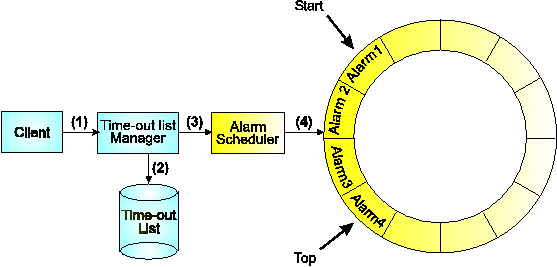
\includegraphics[width=.7\textwidth]{tomarch.png}}

%\vspace*{-0.5in}
\begin{description}
\item[(1)] Client sends requests to TOLM
\item[(2)] TOLM updates its time-out list
\item[(3)] When a time-out expires, TOLM sends an alarm request to \AS
\item[(4)] The \AS{} choses an alarm server---or waits for any
\end{description}





%%%%%%%%%%%%%%%%%%%%%%%%%%%%%%
\end{frame}
\begin{frame}[fragile]{Class TOM --- API}
%%%%%%%%%%%%%%%%%%%%%%%%%%%%%%
\noindent
\begin{tabbing}
{\bf 001} \= tom\UNDSCR{}declare(\&t1, \= 000000000 \= 0000 \kill\\
{\bf 1.}\>  /* declarations */\\
        \> TOM *tom; /* tom is the time-out manager descriptor */\\
        \> timeout\UNDSCR{}t t1, t2; /* two time-out objects, t1 and t2 */\\
        \> int my\UNDSCR{}alarm(TOM*), another\UNDSCR{}alarm(TOM*); /* two alarms */
\end{tabbing}


%%%%%%%%%%%%%%%%%%%%%%%%%%%%%%
\end{frame}
\begin{frame}[fragile]{Class TOM --- API}
%%%%%%%%%%%%%%%%%%%%%%%%%%%%%%
\noindent
\begin{tabbing}
{\bf 001} \= tom\UNDSCR{}declare(\&t1, \= 000000000 \= 0000 \kill\\
{\bf 2.}\> /* definitions */\\
        \> tom $\leftarrow$ tom\UNDSCR{}init(my\UNDSCR{}alarm);\\
        \> tom\UNDSCR{}declare(\&t1, TOM\UNDSCR{}NON\UNDSCR{}CYCLIC, TOM\UNDSCR{}SET\UNDSCR{}ENABLE, \\
        \>                 \> TIMEOUT1, DEADLINE1);  \\
        \> tom\UNDSCR{}declare(\&t2, TOM\UNDSCR{}CYCLIC, TOM\UNDSCR{}SET\UNDSCR{}DISABLE, \\
        \>                 \> TIMEOUT2, DEADLINE2);  \\
        \> tom\UNDSCR{}set\UNDSCR{}action(\&t2, another\UNDSCR{}alarm);
\end{tabbing}



%%%%%%%%%%%%%%%%%%%%%%%%%%%%%%
\end{frame}
\begin{frame}[fragile]{Class TOM --- API}
%%%%%%%%%%%%%%%%%%%%%%%%%%%%%%
\noindent
\begin{tabbing}
{\bf 001} \= tom\UNDSCR{}declare(\&t1, \= 000000000 \= 0000 \kill\\
{\bf 3.}\> /* insertion */\\
        \> tom\UNDSCR{}insert(tom, \&t1), \\
        \> tom\UNDSCR{}insert(tom, \&t2); \\
{\bf 4.}\> /* control */\\
        \> tom\UNDSCR{}enable(tom, \&t2); \\
        \> tom\UNDSCR{}set\UNDSCR{}deadline(\&t2, NEW\UNDSCR{}DEADLINE2); \\
        \> tom\UNDSCR{}renew(tom, \&t2); \\
        \> tom\UNDSCR{}delete(tom, \&t1); \\
        %\\
{\bf 5.}\> /* deactivation */\\
        \> tom\UNDSCR{}close(tom);
\end{tabbing}




%%%%%%%%%%%%%%%%%%%%%%%%%%%%%%
\end{frame}
\begin{frame}[fragile]{Class TOM --- Server-side management}
%%%%%%%%%%%%%%%%%%%%%%%%%%%%%%
\noindent
The time-out list is managed so that
\begin{itemize}
\item The top entry is the closest-to-expiration
\item All the other entries' deadlines are relative
	to the expiration of the top entry
\item A server-side protocol is used to adjust
	the list when inserting / deleting an entry
	from the top / middle / end of the list
\end{itemize}




%%%%%%%%%%%%%%%%%%%%%%%%%%%%%%
\end{frame}
\begin{frame}[fragile]{Class TOM --- Server-side management}
%%%%%%%%%%%%%%%%%%%%%%%%%%%%%%
\noindent
%\centerline{\psfig{figure=tom1.eps,width=19.0cm}}
\centerline{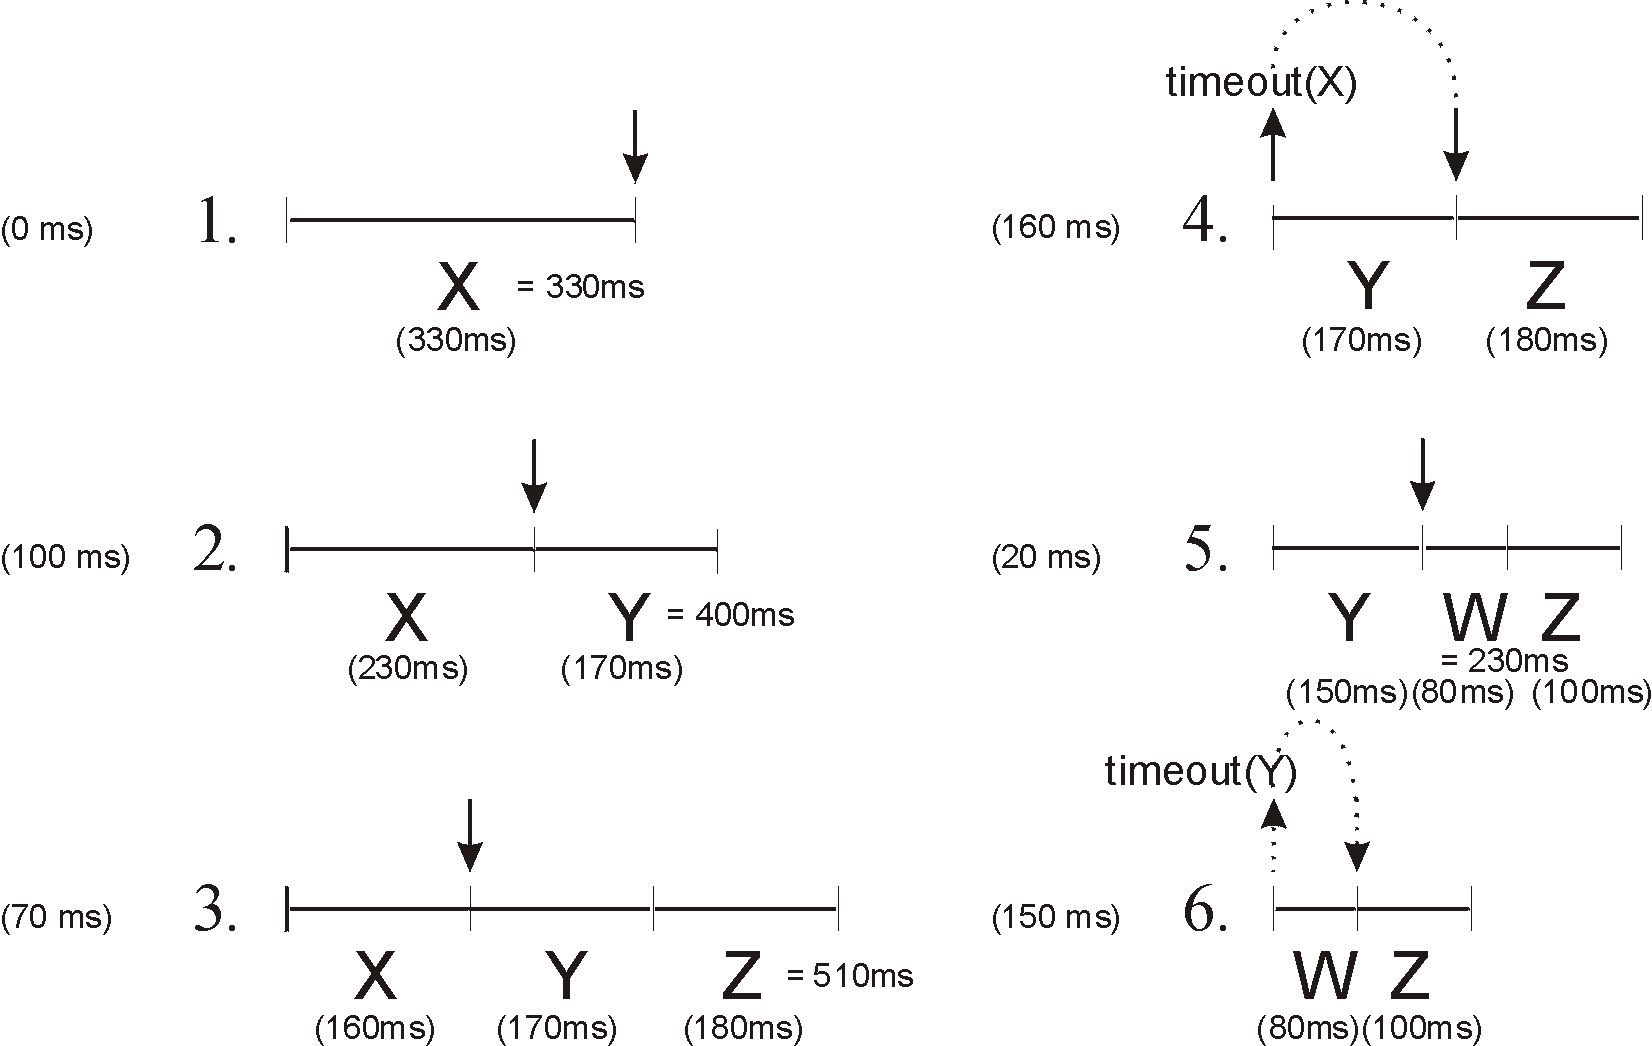
\includegraphics[width=.9\textwidth]{tom1.png}}




%%%%%%%%%%%%%%%%%%%%%%%%%%%%%
\end{frame}
\begin{frame}[fragile]{Class TOM --- Congestion}
%%%%%%%%%%%%%%%%%%%%%%%%%%%%%
\noindent
Problems:

\vspace{20pt}

\begin{itemize}
\item Time-out management implies a delay
\item Time-out detection delay is not always negligible
\item Effect of concurrent execution on the same node
\item \emph{Alarm execution delay is not negligible}
\end{itemize}




%%%%%%%%%%%%%%%%%%%%%%%%%%%%%
\end{frame}
\begin{frame}[fragile]{Class TOM --- Congestion}
%%%%%%%%%%%%%%%%%%%%%%%%%%%%%
\noindent
Alarm $\equiv$ a big source of non determinism:

\vspace{20pt}

\begin{itemize}
  \item It is defined by the user $\Rightarrow$ unknown duration
  \item Alarm often triggers some communication $\Rightarrow$ communication and
	synchronisation delays
  \item Alarms compete with each other, e.g., for a memory port or a channel
\end{itemize}
\end{frame}
%%%%%%%%%%%%%%%%%%%%%%%%%%%%%
\begin{frame}[fragile]{Class TOM --- Congestion}
%%%%%%%%%%%%%%%%%%%%%%%%%%%%%
\begin{description}
\item[$\Rightarrow$ Risk]: non negligible delay between
\end{description}


\vspace{20pt}

\[
     t_{\hbox{\small expiration}} \qquad \hbox{ and } \qquad t_{\hbox{\small alarm execution}}
\]


\vspace{20pt}

\begin{description}
\item[$\Rightarrow$ Need]: a way is needed

     \begin{itemize}
     \item to manifest, \ 
     
     \hspace*{50pt} and, if possible,
     \item to keep under control
     \end{itemize} 
     the \textbf{congestion} that is due to concurrent alarm execution.
\end{description}




%%%%%%%%%%%%%%%%%%%%%%%%%%%%%
\end{frame}
\begin{frame}[fragile]{Class TOM --- Congestion}
%%%%%%%%%%%%%%%%%%%%%%%%%%%%%
\noindent
TOM supports multiple alarm execution threads.

\vspace{20pt}

\begin{itemize}
  \item Does this solve the problem of congestion?  
  \item (Are there cases in which the problem is solved, or 
  at least, softened?)
\end{itemize}

%\noindent
%TOM works at discrete time steps: every 
%{\sf TOM\UNDSCR{}CYCLE} clock ticks, it checks whether
%something has changed and requires adjustment


%%%%%%%%%%%%%%%%%%%%%%%%%%%%%
\end{frame}
\begin{frame}[fragile]{Class TOM --- Congestion}
%%%%%%%%%%%%%%%%%%%%%%%%%%%%%
\noindent
Experiments have been performed.

\noindent
Variables: 
\begin{itemize}
\item alarm latency ($\delta$),
\item time-out deadline,
\item number of alarm threads ($\tau$),
\item \emph{competition}.
\end{itemize}


\vspace{20pt}

\noindent
{\sf TOM\_CYCLE} = 50000 clock ticks (50ms).


\vspace{20pt}

\noindent
Output: actual time of alarm minus expected time of alarm.


%%%%%%%%%%%%%%%%%%%%%%%%%%%%%
\end{frame}
\begin{frame}[fragile]{Class TOM --- Congestion}
%%%%%%%%%%%%%%%%%%%%%%%%%%%%%
\noindent
Experiment 1:
\begin{itemize}
\item $\delta\approx50\mu\hbox{s}$
\item Deadline: uniform in $[0,T]$
\item Single alarm thread
\item No competition (alarms execute \textsf{sleep()} )
\end{itemize}


\vspace{20pt}

\noindent
Deadline=50$\mu\hbox{s}$ = overhead for calling a function and copying a
20-byte message on
a DEC Alpha board running the TEX o.s.



%%%%%%%%%%%%%%%%%%%%%%%%%%%%%
\end{frame}
\begin{frame}[fragile]{Class TOM --- Congestion}
%%%%%%%%%%%%%%%%%%%%%%%%%%%%%
\noindent
%\centerline{\psfig{figure=./delays-t100-a0.ps,angle=-90,width=15.0cm}}
\centerline{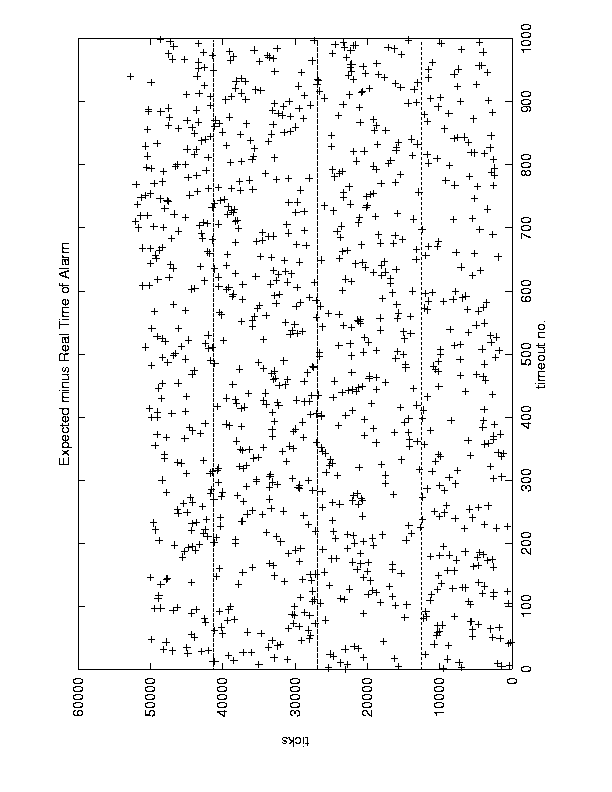
\includegraphics[width=.7\textwidth,angle=-90]{delays-t100-a0.png}}

%%%%%%%%%%%%%%%%%%%%%%%%%%%%%
\end{frame}
\begin{frame}[fragile]{Class TOM --- Congestion}
%%%%%%%%%%%%%%%%%%%%%%%%%%%%%
\begin{itemize}
\item Max=52787, min=157, avg=26892.74, stdev=14376.89
\item 20 $>$ {\sf TOM\UNDSCR{}CYCLE}
\end{itemize}

%\vfill
%\eject
%\leftheader{ }
%\rightheader{ }

%%%%%%%%%%%%%%%%%%%%%%%%%%%%%
\end{frame}
\begin{frame}[fragile]{ }
%%%%%%%%%%%%%%%%%%%%%%%%%%%%%
\noindent
%\hspace*{-0.6in}\vspace*{-1.3in}%
%\vbox{\hbox{\psfig{figure=./delays-t100-a5000.ps,angle=-90,width=13.0cm}%
%\psfig{figure=./delays-t100-a10000.ps,angle=-90,width=13.0cm}}
%\vskip-0.4in\hspace*{2.0in}\vspace*{-2.4in}\hbox{\vspace*{-1.3in}\psfig{figure=./delays-t100-a20000.ps,angle=-90,width=13.0cm}}}
%

\centerline{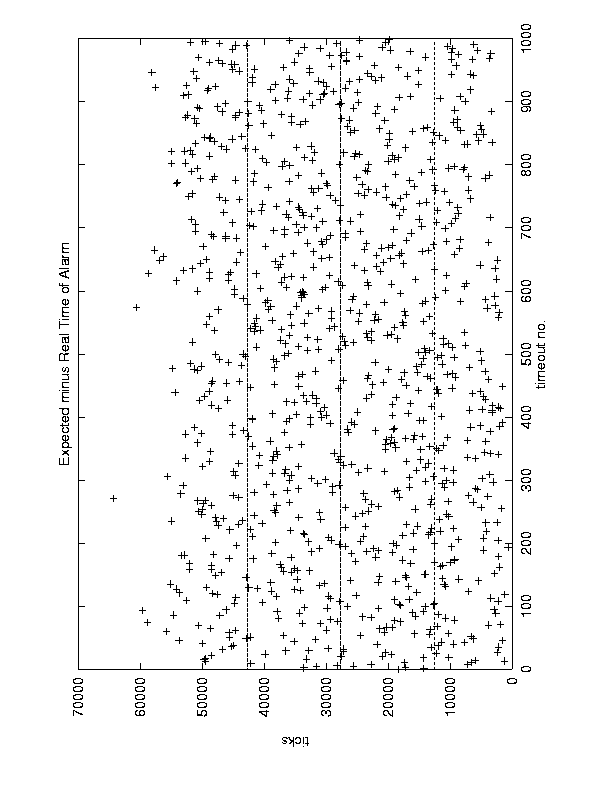
\includegraphics[width=.7\textwidth,angle=-90]{delays-t100-a5000.png}}
\end{frame}
\begin{frame}[fragile]{ }
\centerline{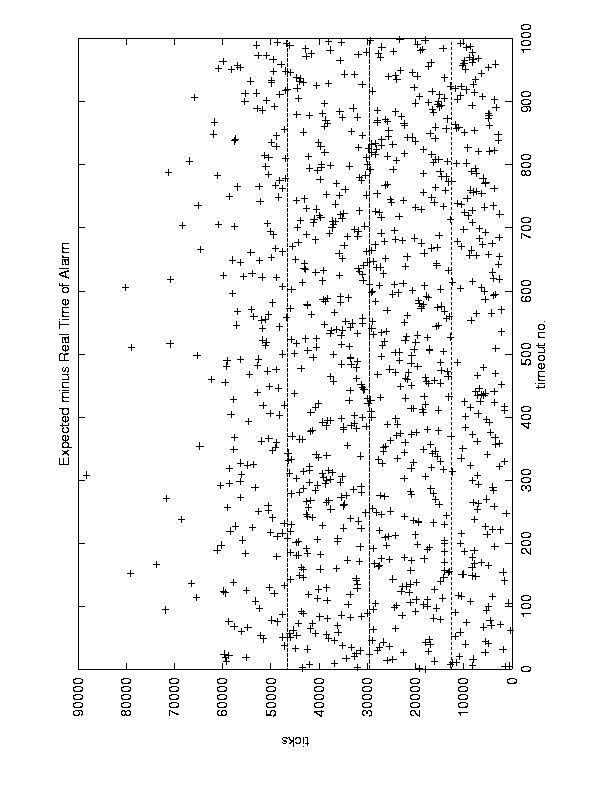
\includegraphics[width=.7\textwidth,angle=-90]{delays-t100-a10000.png}}
\end{frame}
\begin{frame}[fragile]{ }
\centerline{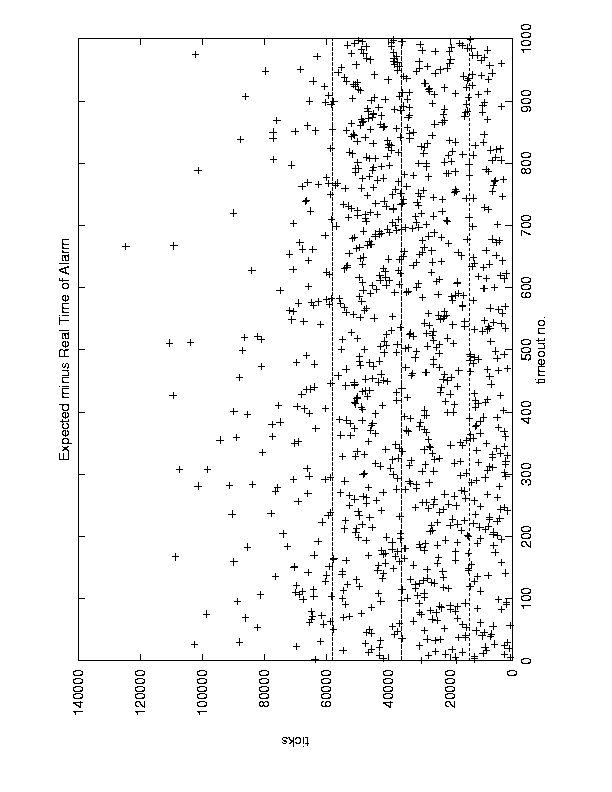
\includegraphics[width=.7\textwidth,angle=-90]{delays-t100-a20000.png}}
\end{frame}

%%%%%%%%%%%%%%%%%%%%%%%%%%%%%
\begin{frame}[fragile]{Class TOM --- Congestion}
%%%%%%%%%%%%%%%%%%%%%%%%%%%%%
\noindent
%\centerline{\psfig{figure=cmp1.ps,angle=-90,width=15.0cm}}
\centerline{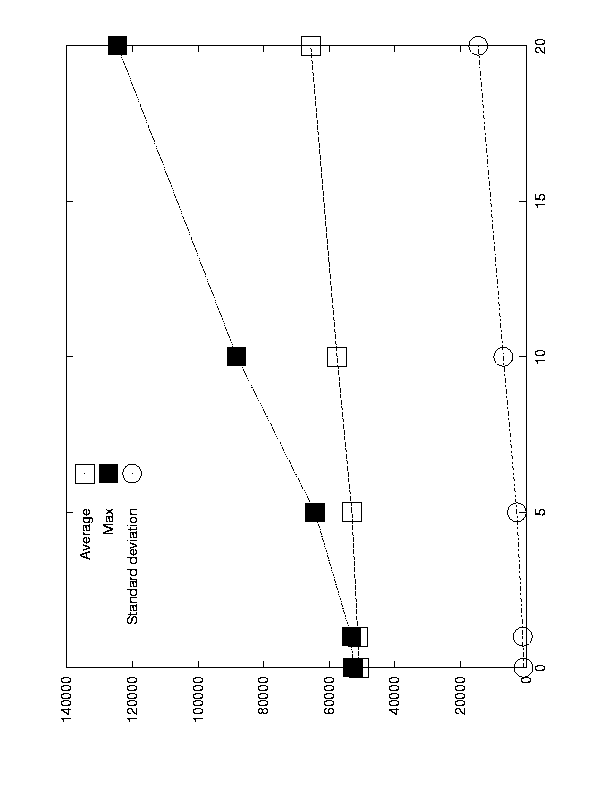
\includegraphics[width=.7\textwidth,angle=-90]{cmp1.png}}

%\vfill
%\eject
%\leftheader{ }
%\rightheader{ }

\end{frame}
%%%\begin{frame}[fragile]{ }
%%%\centerline{\includegraphics[width=.5\textwidth,angle=-90]{chaos-060.png}}
%%%\end{frame}
%%%\begin{frame}[fragile]{ }
%%%\centerline{\includegraphics[width=.5\textwidth,angle=-90]{chaos-080.png}}
%%%\end{frame}
%%%\begin{frame}[fragile]{ }
%%%\centerline{\includegraphics[width=.5\textwidth,angle=-90]{chaos-090.png}}
%%%\end{frame}
%%%\begin{frame}[fragile]{ }
%%%
%%%%%%%%%%%%%%%%%%%%%%%%%%%%%%%%
%%%\end{frame}
\begin{frame}[fragile]{ }
%%%%%%%%%%%%%%%%%%%%%%%%%%%%%
\noindent
%%\hspace*{-0.6in}\vspace*{-1.3in}%
%%\vbox{\hbox{\psfig{figure=./chaos-100.ps,angle=-90,width=13.0cm}%
%%\psfig{figure=./chaos-100-1.ps,angle=-90,width=13.0cm}}
%%\vskip-0.4in\hspace*{2.0in}\vspace*{-2.4in}\hbox{\vspace*{-1.3in}\psfig{figure=./chaos-100-2.ps,angle=-90,width=13.0cm}}}
%%
\centerline{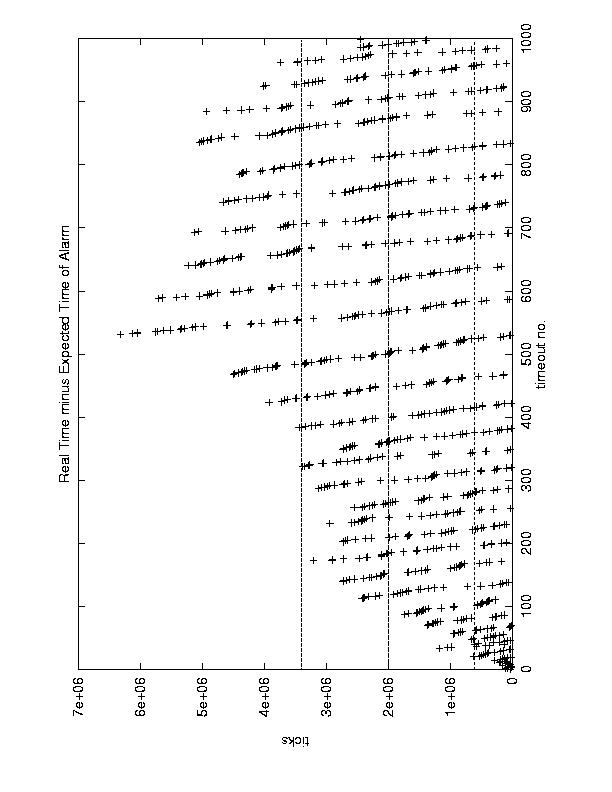
\includegraphics[width=.7\textwidth,angle=-90]{chaos-100.png}}
\end{frame}
\begin{frame}[fragile]{ }
\centerline{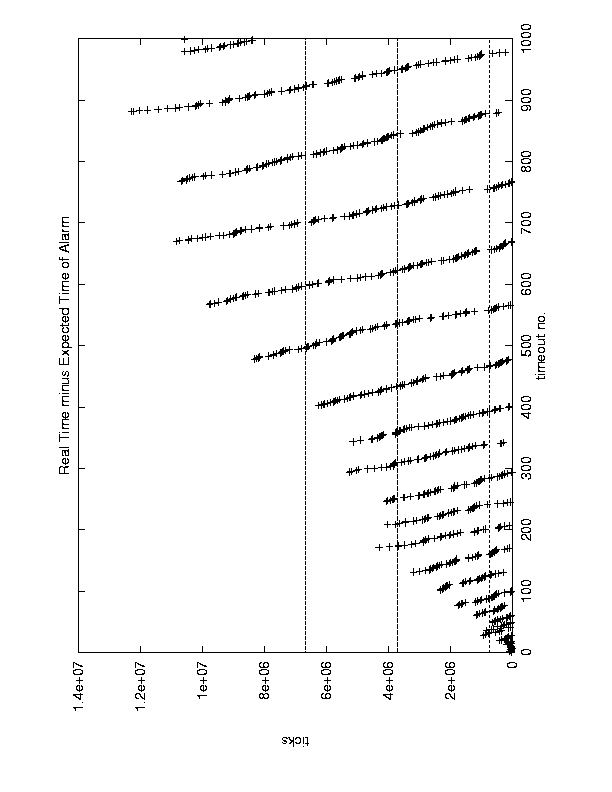
\includegraphics[width=.7\textwidth,angle=-90]{chaos-100-1.png}}
\end{frame}
%%%\begin{frame}[fragile]{ }
%%%\centerline{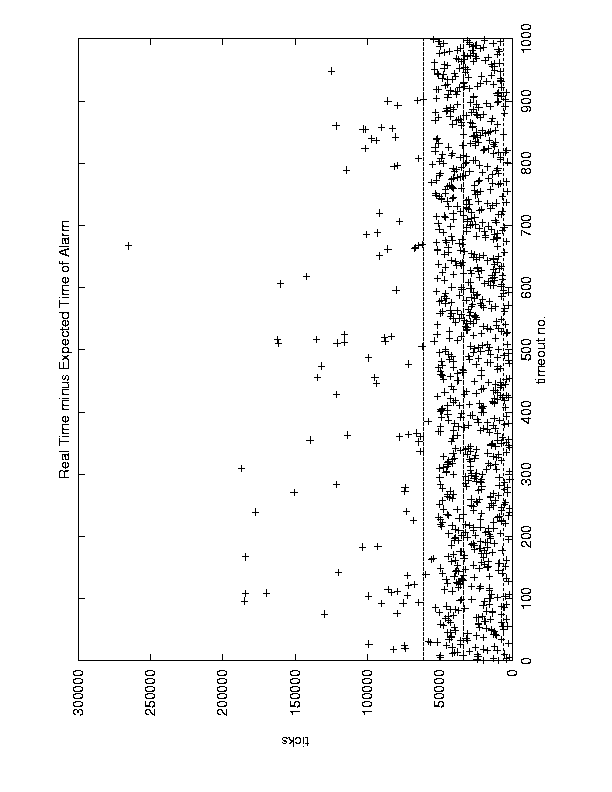
\includegraphics[width=.5\textwidth,angle=-90]{chaos-100-2.png}}
%%%\end{frame}
\begin{frame}[fragile]{ }
%%%%%%%%%%%%%%%%%%%%%%%%%%%%%
\noindent
\centerline{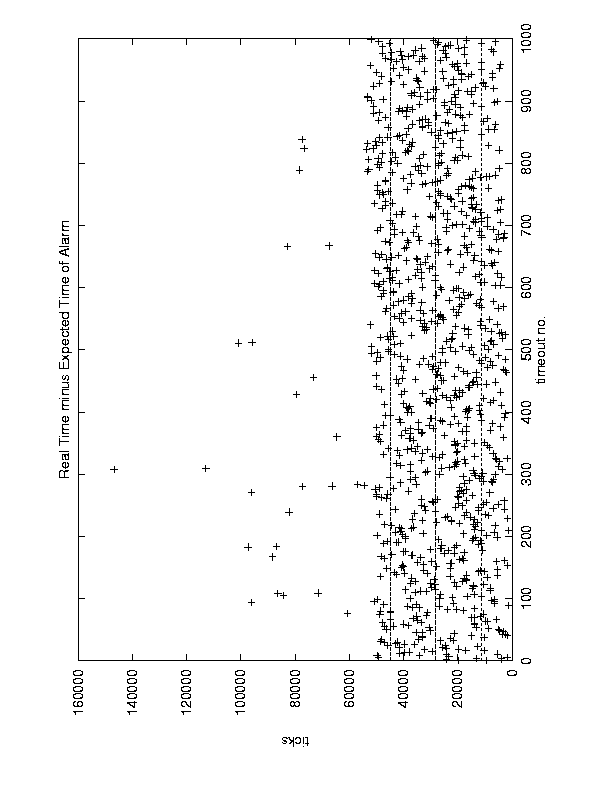
\includegraphics[width=.7\textwidth,angle=-90]{chaos-100-3.png}}
\end{frame}
\begin{frame}[fragile]{ }
\centerline{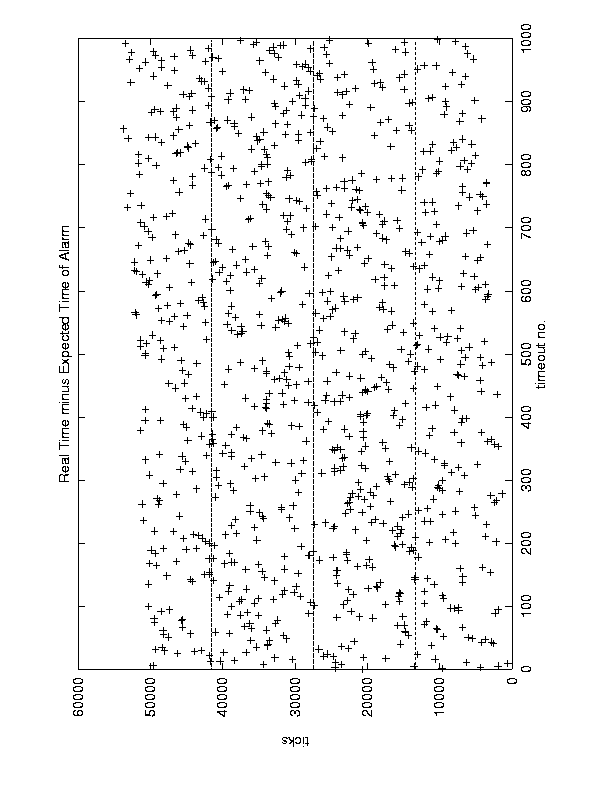
\includegraphics[width=.7\textwidth,angle=-90]{chaos-100-5.png}}
%\psfig{figure=./chaos-100-3.ps,angle=-90,width=14.0cm}
%\psfig{figure=./chaos-100-5.ps,angle=-90,width=14.0cm}


%%%%%%%%%%%%%%%%%%%%%%%%%%%%%
\end{frame}
\begin{frame}[fragile]{Class TOM --- Congestion}
%%%%%%%%%%%%%%%%%%%%%%%%%%%%%


\vspace{20pt}

\noindent
\begin{small}
\begin{tabular}{c|l|l|l|l|l|l}
$\tau$&$\mu$&$\sigma$&$exce-$&max&$\mu'$&$\sigma'$\\
&&&$ptions$&&&\\\hline
1&3692158.86&2966039.23&974&12277216&3790057.80&2943375.88\\
2&33674.46&27688.17&140&264882&83244.94&38052.06\\
3&28177.01&16801.97&54&146684&66737.87&20705.76\\
4&27621.63&14276.78&45&100260&52871.73&7358.90\\
5&27435.40&14087.22&44&53712&51375.93&1001.36\\
6&27475.84&14107.32&44&53992&51443.95&1008.77\\ \hline
\end{tabular}
\end{small}

\begin{itemize}
\item $\mu$ and $\sigma$ = average and stdev of the 1000 outcomes.
\item $\mu'$ and $\sigma'$ = average and stdev of the exceptions
\end{itemize}


%%%%%%%%%%%%%%%%%%%%%%%%%%%%%
\end{frame}
\begin{frame}[fragile]{Class TOM --- Congestion}
%%%%%%%%%%%%%%%%%%%%%%%%%%%%%
\noindent
Congestion as a result of competition! (Alarms compete for the CPU). $\delta=20$ms.


\vspace{20pt}

\begin{tabular}{c|l|l|l|l|l|l}
$\tau$&$\mu$&$\sigma$&$\gamma$&max&$\mu'$&$\sigma'$\\ \hline
1&35251.93&21667.08&226&126931&66223.70&13713.40\\
2&35533.45&21584.35&248&127403&64377.88&13803.45\\ 
3&35735.19&21606.70&250&125910&64681.21&13305.83\\ \hline
\end{tabular}


\vspace{20pt}

Conclusion: in the worst case adding alarm executors \emph{does not\/}
influence congestion!


%%%%%%%%%%%%%%%%%%%%%%%%%%%%%
\end{frame}
\begin{frame}[fragile]{Class TOM --- Congestion}
%%%%%%%%%%%%%%%%%%%%%%%%%%%%%
\noindent
Solutions: resource-specific. 
\begin{itemize}
\item Multicore CPU 
      that dynamically
      and transparently schedules the parallel execution of alarms
      on the available cores.
\item I/O $\Rightarrow$
      parallel I/O systems.
\end{itemize}


%%%%%%%%%%%%%%%%%%%%%%%%%%%%%
\end{frame}
\begin{frame}[fragile]{Class TOM --- Case Study: the Backbone}
%%%%%%%%%%%%%%%%%%%%%%%%%%%%%
\noindent
The backbone: a distributed middleware for fault-tolerant embedded
applications.


\vspace{20pt}

\noindent 
The backbone tolerates crash failures of nodes and backbone components.


\vspace{20pt}

\noindent
Based on TOM:
\begin{itemize}
\item IA\_SET\_TIMEOUT, IA\_CLEAR\_TIMEOUT
\item MIA\_SEND\_TIMEOUT, TAIA\_RECV\_TIMEOUT
\item MIA\_RECV\_TIMEOUT, TAIA\_SEND\_TIMEOUT
\end{itemize}


%%%%%%%%%%%%%%%%%%%%%%%%%%%%%
\end{frame}
\begin{frame}[fragile]{Class TOM --- Conclusion}
%%%%%%%%%%%%%%%%%%%%%%%%%%%%%
\noindent
\begin{itemize}
\item Application-level time-out support
\item Available on Windows, Parsytec EPX, TEX microkernel
\item Multi-threaded architectures $\Rightarrow$ better exploitment
      of a system's resources
\item Problem of congestion due to the concurrent execution of alarms
\item Successfully used in European projects
\item ``Algorithm of mutual suspicion''
\end{itemize}


%%%%%%%%%%%%%%%%%%%%%%%%%%%%%%%%%%%%%%%%%%%%%%%
\end{frame}
\begin{frame}[fragile]{Class FN}
\begin{itemize}
\item FN : a class for application-level input and interpretation of user-defined
      functions
\item The user types in a mathematical function. This function can be then be evaluated.
\item See \verb"https://github.com/Eidonko/FN"
\item Same principle and shape of class FILE:
\end{itemize}

\vspace{20pt}

\begin{verbatim}
FN *f;     double *x, *y, z; float d;
printf("Please, type in a function of variables x and y\n");
f = fnopen();
\end{verbatim}


%%%%%%%%%%%%%%%%%%%%%%%%%%%%%%%%%%%%%%%%%%%%%%%
\end{frame}
\begin{frame}[fragile]{Class FN}
\begin{verbatim}
/* x and y point resp. to variables FN.x and FN.y */
x = fnmemory(f, 'x');
y = fnmemory(f, 'y');

printf("Please, type in a value for x and a value for y\n");
scanf("%f", &d); *x = d;
scanf("%f", &d); *y = d;

printf("The value of your function in %lf and %lf is %lf\n",
       *x, *y, fnread());
\end{verbatim}



%%%%%%%%%%%%%%%%%%%%%%%%%%%%%%%%%%%%%%%%%%%%%%%
\end{frame}
\begin{frame}[fragile]{Class FN}
\begin{itemize}
\item Written with LEX and YACC
\item Test program on the web: Julia sets
\item Example: julia -1 1 -1 1 200, re(x,y)=x*x-y*y, im(x,y)=2*x*y+0.99) 
\end{itemize}
\end{frame}
%%%%%%%%%%%%%%%%%%%%%%%%%%%%%%%%%%%%%%%%%%%%%%%
